% DOCUMENT CLASS
%%%%%%%%%%%%%%%%%%%%%%%%%%%%%%%%%%%%%%%%%%%%%%%%%%%%%%%%%%%%%%%%%%%%%%%%%%%%%%%%%%%%%%%%%%%%%%%%%%%%%%

\documentclass[journal=jacsat,manuscript=article]{achemso}
\SectionNumbersOn  % This is necessary to use section labels and referencing with ACS template.

% Single-spaced, two-column with PRL look and style (easy on the eyes)
%\documentclass[aps,pre,twocolumn,nofootinbib,superscriptaddress,linenumbers]{revtex4-1}

%\documentclass[aip, jcp, reprint]{revtex4-1}  % arxiv version
\pdfoutput=1  % for arxiv

% Double-spaced, one-column style (for submission/review/editing)
%\documentclass[aps,preprint,prl,superscriptaddress,showpacs]{revtex4}

%%%%%%%%%%%%%%%%%%%%%%%%%%%%%%%%%%%%%%%%%%%%%%%%%%%%%%%%%%%%%%%%%%%%%%%%%%%%%%%%%%%%%%%%%%%%%%%%%%%%%%
% PREAMBLE
%%%%%%%%%%%%%%%%%%%%%%%%%%%%%%%%%%%%%%%%%%%%%%%%%%%%%%%%%%%%%%%%%%%%%%%%%%%%%%%%%%%%%%%%%%%%%%%%%%%%%%

% FONT
% Change to a sans serif font for submission.  Comment out for arxiv.
%\usepackage{sourcesanspro}  % Comment out this and the next line for submission to ACS journal.
%\renewcommand*\familydefault{\sfdefault} %% Only if the base font of the document is to be sans serif
%
%\usepackage[T1]{fontenc}
%\usepackage[font=sf,justification=justified]{caption}
%\usepackage[font=sf]{floatrow}  % Disabled for ACS

% Rework captions to use sans serif font.  % Commented out for ACS
%\makeatletter	
%\renewcommand\@make@capt@title[2]{%
% \@ifx@empty\float@link{\@firstofone}{\expandafter\href\expandafter{\float@link}}%
%  {\sf\textbf{#1}}\sf\@caption@fignum@sep#2\quad
%}%
%\makeatother

\usepackage{amsmath}
\usepackage{amssymb}
\usepackage{graphicx}
\usepackage{caption}
%\usepackage{dcolumn}
\usepackage{boxedminipage}
\usepackage{verbatim}
\usepackage{booktabs}
\usepackage{subfigure}
\usepackage{listings}

%\usepackage[colorlinks=true,citecolor=blue,linkcolor=blue]{hyperref}  % Commented out to remove colors per ACS requirements.

% The figures are in a figures/ subdirectory.
%\graphicspath{{../figures/}}

%\bibliographystyle{apsrevlong}
\bibliographystyle{apsrev}

% italicized boldface for math (e.g. vectors)
\newcommand{\bfv}[1]{{\mbox{\boldmath{$#1$}}}}
% non-italicized boldface for math (e.g. matrices)
\newcommand{\bfm}[1]{{\bf #1}}          

% Pretty-printing of shell commands
\newcommand{\shellcmd}[1]{\\\ \texttt{\scriptsize\# #1}\\}

%\newcommand{\bfm}[1]{{\mbox{\boldmath{$#1$}}}}
%\newcommand{\bfm}[1]{{\bf #1}}
\newcommand{\expect}[1]{\left \langle #1 \right \rangle}                % <.> for denoting expectations over realizations of an experiment or thermal averages
\newcommand{\dhdl}{\frac{dH}{d\lambda}}
% vectors
\newcommand{\var}[1]{{\mathrm var}{(#1)}}
\newcommand{\x}{\bfv{x}}
\newcommand{\y}{\bfv{y}}
\newcommand{\f}{\bfv{f}}

\newcommand{\bfc}{\bfm{c}}
\newcommand{\hatf}{\hat{f}}

\newcommand{\bTheta}{\bfm{\Theta}}
\newcommand{\btheta}{\bfm{\theta}}
\newcommand{\bhatf}{\bfm{\hat{f}}}
\newcommand{\Cov}[1] {\mathrm{cov}\left( #1 \right)}
\newcommand{\Ept}[1] {{\mathrm E}\left[ #1 \right]}
\newcommand{\Eptk}[2] {{\mathrm E}_{#1}\left[ #2\right]}
\newcommand{\T}{\mathrm{T}}                                % T used in matrix transpose

\renewcommand{\thefigure}{S\arabic{figure}}  % Make figures say Fig. S1

%%%%%%%%%%%%%%%%%%%%%%%%%%%%%%%%%%%%%%%%%%%%%%%%%%%%%%%%%%%%%%%%%%%%%%%%%%%%%%%%
% DOCUMENT
%%%%%%%%%%%%%%%%%%%%%%%%%%%%%%%%%%%%%%%%%%%%%%%%%%%%%%%%%%%%%%%%%%%%%%%%%%%%%%%%


%%%%%%%%%%%%%%%%%%%%%%%%%%%%%%%%%%%%%%%%%%%%%%%%%%%%%%%%%%%%%%%%%%%%%%%%%%%%%%%%
% TITLE AND AUTHORS
%%%%%%%%%%%%%%%%%%%%%%%%%%%%%%%%%%%%%%%%%%%%%%%%%%%%%%%%%%%%%%%%%%%%%%%%%%%%%%%%

\title{Supporting Information for Towards Automated Benchmarking of Atomistic Forcefields:\\
Neat Liquid Densities and Static Dielectric Constants from the ThermoML Data Archive}

\author{Kyle A. Beauchamp$^+$}
%\thanks{Corresponding author}  % Disabled for ACS
\email{kyle.beauchamp@choderalab.org}
\affiliation{Computational Biology Program, Sloan Kettering Institute, Memorial Sloan Kettering Cancer Center, New York, NY}

\author{Julie M. Behr$^+$}
%\email{julie.behr@choderalab.org}
\affiliation{Tri-Institutional Program in Computational Biology and Medicine, Weill Cornell Medical College, New York, NY}

\author{Ari\"{e}n S. Rustenburg}
%\email{bas.rustenburg@choderalab.org}
\affiliation{Graduate Program in Physiology, Biophysics, and Systems Biology, Weill Cornell Medical College, New York, NY}
 
 \author{Christopher I. Bayly}
% \email{bayly@eyesopen.com}
 \affiliation{OpenEye Scientific Software Inc., Santa Fe, NM}
 
 
 \author{Kenneth Kroenlein}
% \email{kenneth.kroenlein@nist.gov}
 \affiliation{Thermodynamics Research Center, NIST, Boulder, CO}
 
 \author{John D. Chodera}
%\thanks{Corresponding author}  % Disabled for ACS
 \email{john.chodera@choderalab.org}
 \affiliation{Computational Biology Program, Sloan Kettering Institute, Memorial Sloan Kettering Cancer Center, New York, NY}

\date{\today}

\begin{document}  % For ACS, had to move begin document to after the author info



\section{Supporting Information}

\begin{itemize}
 \item Figure: Timestep-dependence of density
 \item Figure: Error analysis (density) for ThermoML dataset
 \item Figure: Error analysis (static dielectric constant) for ThermoML dataset
 \item Figure: Temperature Dependence: Density
 \item Figure: Temperature Dependence: Static Dielectric Constant
 \item Commands to install dependencies
\end{itemize}

\clearpage


\begin{figure}

\subfigure[]{
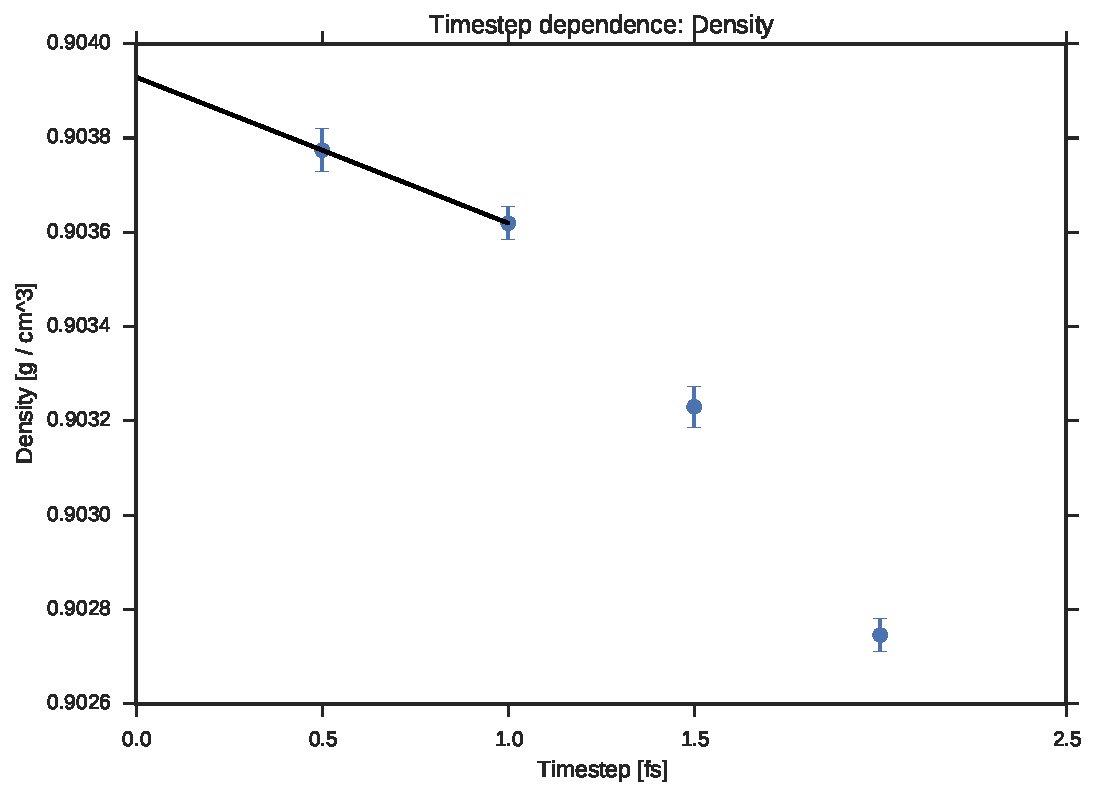
\includegraphics[width=8cm]{./figures/timestep_dependence_density.pdf}
}
\subfigure[]{
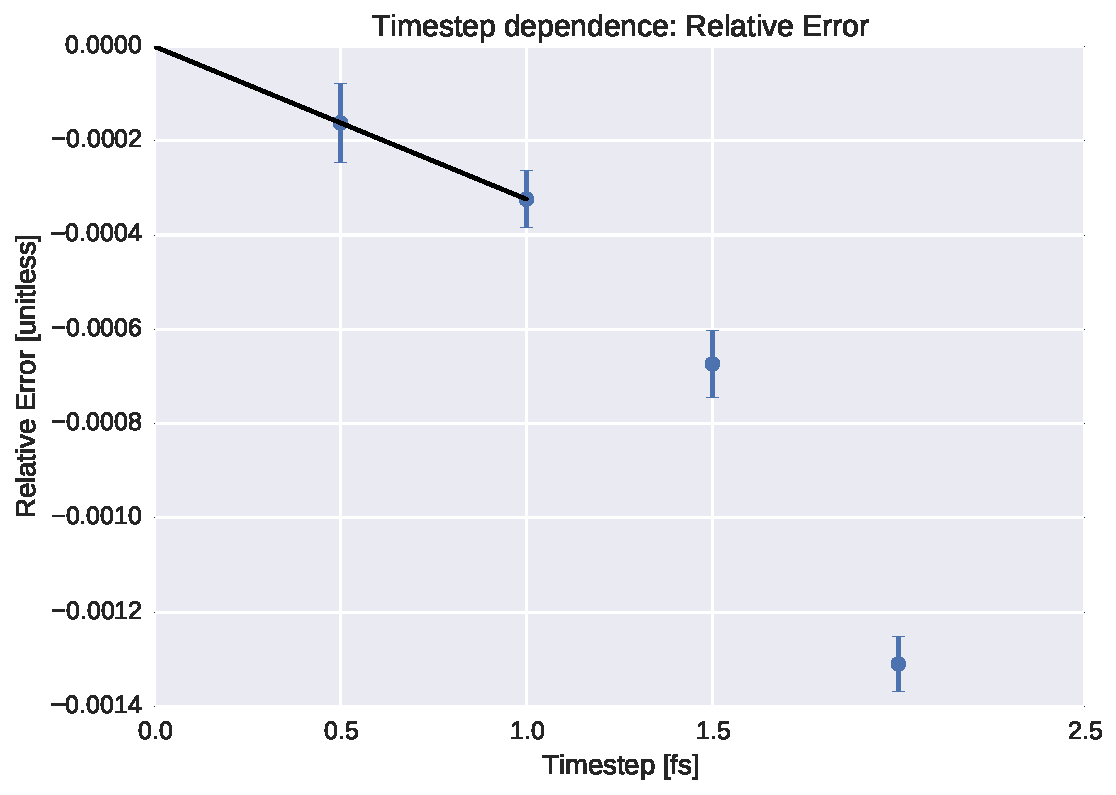
\includegraphics[width=8cm]{./figures/timestep_dependence_relative_error.pdf}
}

\caption{
{\bf Dependence of computed density on simulation timestep.}
To probe the systematic error from finite time-step integration, we examined the timestep dependence of butyl acrylate density.  
(a).  The density is shown for several choices of timestep.  
(b).  The relative error, as compared to the reference value, is shown for several choices of timestep.  
Error bars represent standard errors of the mean, with the number of effective samples estimated using pymbar's statistical inefficiency routine \cite{shirts2008statistically}.  
The reference value is estimated by linear extrapolation to 0 fs using the 0.5 fs and 1.0 fs data points; the linear extrapolation is shown as black lines.  
We find a 2~fs timestep leads to systematic biases in the density on the order of 0.13\%, while 1 fs reduces the systematic bias to approximately 0.03\%---we therefore selected a 1~fs timestep for the present work, where we aimed to achieve three digits of accuracy in density predictions.
}
\label{figure:timestep}

\end{figure}




%%%%%%%%%%%%%%%%%%%%%%%%%%%%%%%%%%%%%%%%%%%%%%%%%%%%%%%%%%%%%%%%%%%%%%%%%%%%%%%%
% Assessment of experimental error
%%%%%%%%%%%%%%%%%%%%%%%%%%%%%%%%%%%%%%%%%%%%%%%%%%%%%%%%%%%%%%%%%%%%%%%%%%%%%%%%

%%%%%%%%%%%%%%%%%%%%%%%%%%%%%%%%%%%%%%%%%%%%%%%%%%%%%%%%%%%%%%%%%%%%%%%%%%%%%%%%
% FIGURE: ILLUSTRATION OF ASSESSMENT OF EXPERIMENTAL ERROR: DENSITY
%%%%%%%%%%%%%%%%%%%%%%%%%%%%%%%%%%%%%%%%%%%%%%%%%%%%%%%%%%%%%%%%%%%%%%%%%%%%%%%%

\clearpage

\begin{figure}

\subfigure[]{
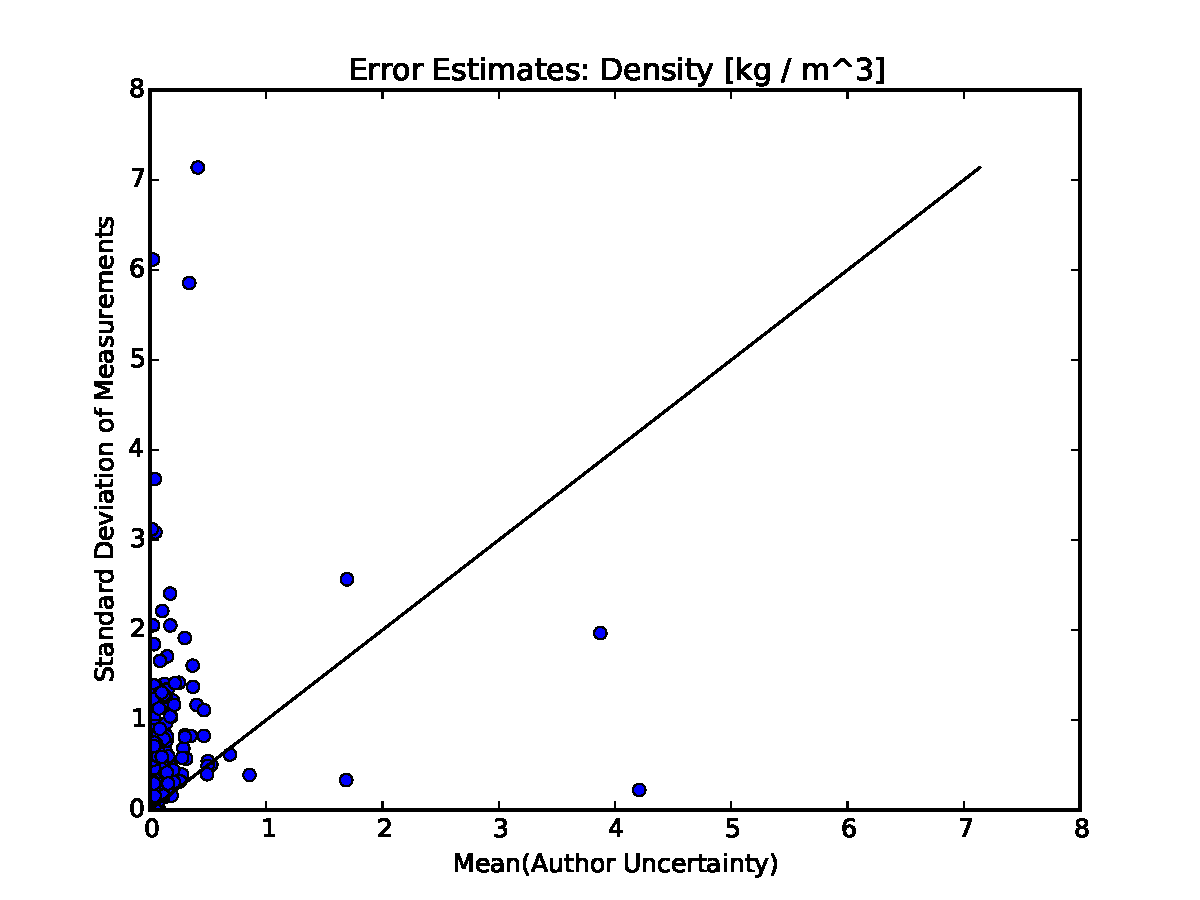
\includegraphics[width=7.3cm]{./figures/error_analysis_density.pdf}
}

\subfigure[]{
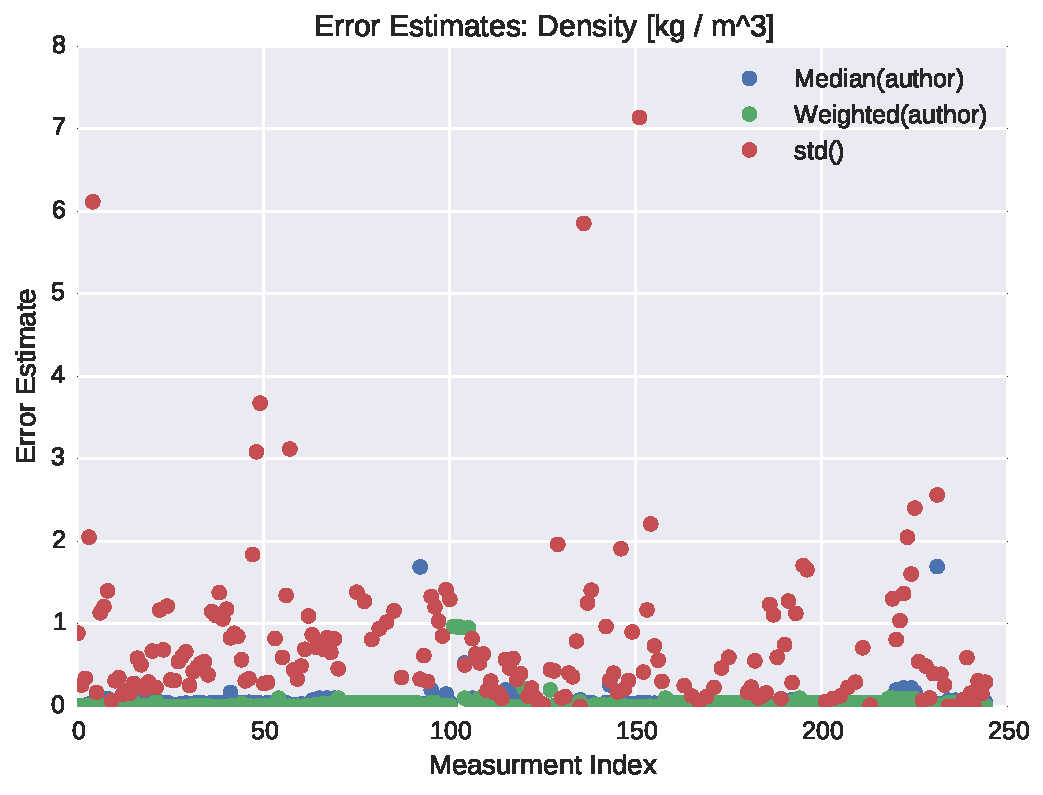
\includegraphics[width=7.3cm]{./figures/error_analysis_density_index.pdf}
}

\caption{{\bf Assessment of experimental error: Density}
To assess the experimental error in our ThermoML extract, we compared three different estimates of uncertainty.  
In the first approach (Weighted), we computed the standard deviation of the optimally weighted average of the measurements, using the uncertainties reported by authors ($\sigma_\textnormal{Weighted} = [\sum_k \sigma_k^{-2}]^{-0.5}$).
This uncertainty estimator places the highest weights on measurements with small uncertainties and is therefore easily dominated by small outliers and uncertainty under-reporting.
In the second approach (Median), we estimated the median of the uncertainties reported by authors; this statistic should be robust to small and large outliers of author-reported uncertainties.
In the third approach (Std), we calculated at the standard deviation of independent measurements reported in the ThermoML extract, completely avoiding the author-reported uncertainties.
Plot (a) compares the three uncertainty estimates.
We see that author-reported uncertainties appear to be substantially smaller than the scatter between the observed measurements.
A simple psychological explanation might be that because density measurements are more routine, the authors simply report the repeatability stated by the manufacturer (e.g.,~0.0001 g/cm$^{3}$ for a Mettler Toledo DM40~\cite{mettlertoledo}).  
However, this hardware limit is not achieved due to inconsistencies in sample preparation and experimental conditions; see Appendix in Ref.~\cite{chirico2013improvement}.  
Panel (b) shows the same information as (a) but as a function of the measurement index, rather than as a scatter plot---because not all measurements have author-supplied uncertainties, panel (c) contains slightly more data points than (a, b).  
%{\color{red}[JDC: Should discuss with Kenneth what kind of story to make out of this, and what to say in the main manuscript body.]}
%KAB: I think the error analysis is now partially discussed in the density sections.
}
\label{figure:ErrorAnalysisDensity}

\end{figure}


%%%%%%%%%%%%%%%%%%%%%%%%%%%%%%%%%%%%%%%%%%%%%%%%%%%%%%%%%%%%%%%%%%%%%%%%%%%%%%%%
% FIGURE: ILLUSTRATION OF ASSESSMENT OF EXPERIMENTAL ERROR: DIELECTRIC
%%%%%%%%%%%%%%%%%%%%%%%%%%%%%%%%%%%%%%%%%%%%%%%%%%%%%%%%%%%%%%%%%%%%%%%%%%%%%%%%

\clearpage



\begin{figure}

\subfigure[]{
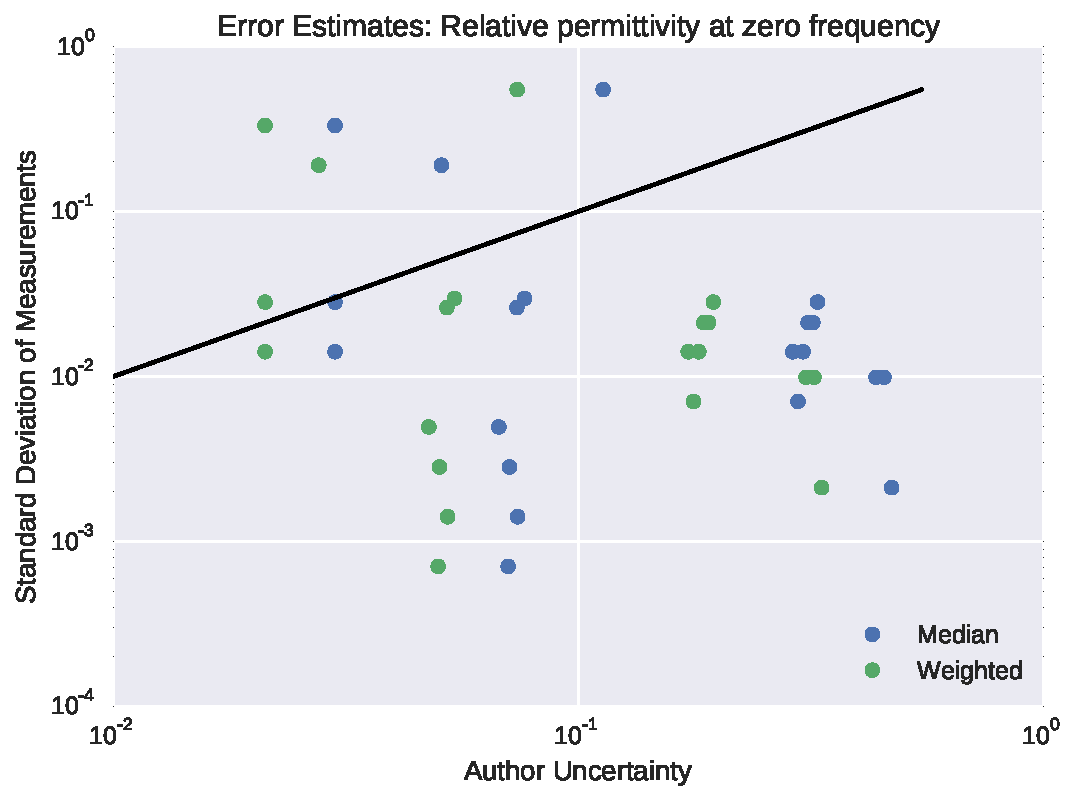
\includegraphics[width=7.3cm]{./figures/error_analysis_dielectric.pdf}
}

\subfigure[]{
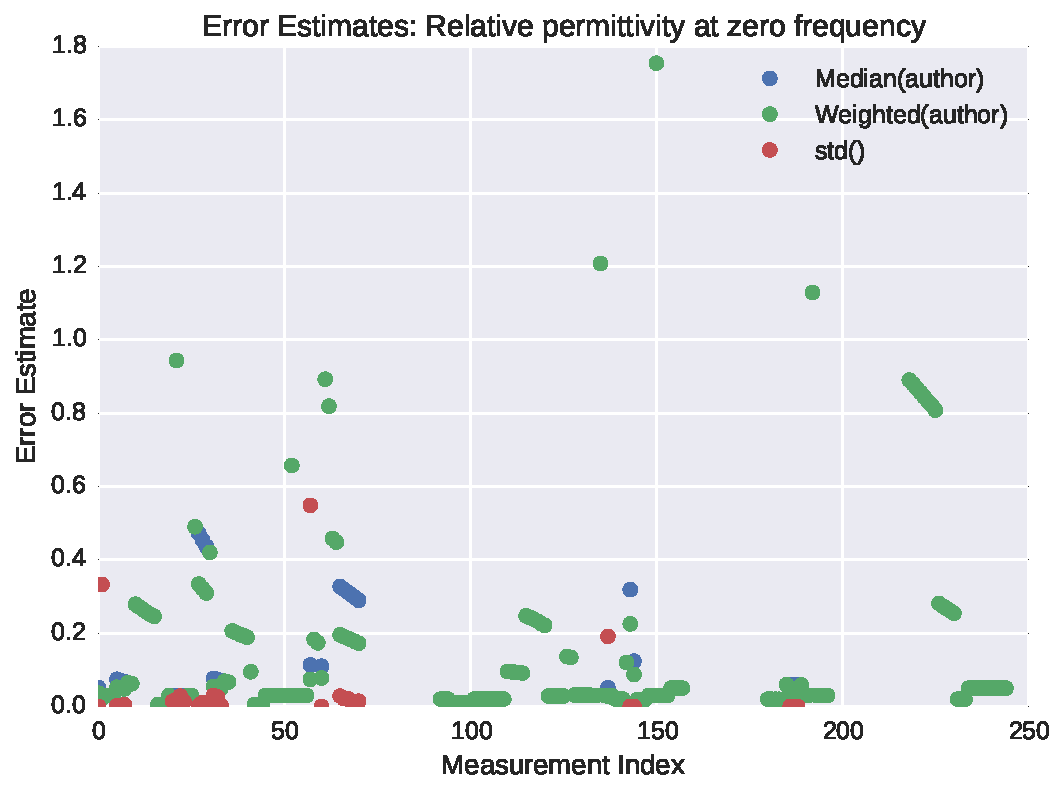
\includegraphics[width=7.3cm]{./figures/error_analysis_dielectric_index.pdf}
}

\caption{{\bf Assessment of experimental error: Static Dielectric Constant}
To assess the experimental error in our ThermoML extract, we compared three different estimates of uncertainty.  
In the first approach (Weighted), we computed the standard deviation of the optimally weighted average of the measurements, using the uncertainties reported by authors ($\sigma_\textnormal{Weighted} = [\sum_k \sigma_k^{-2}]^{-0.5}$).
This uncertainty estimator places the highest weights on measurements with small uncertainties and is therefore easily dominated by small outliers and uncertainty under-reporting.
In the second approach (Median), we estimated the median of the uncertainties reported by authors; this statistic should be robust to small and large outliers of author-reported uncertainties.
In the third approach (Std), we calculated at the standard deviation of independent measurements reported in the ThermoML extract, completely avoiding the author-reported uncertainties.
Plot (a) compares the three uncertainty estimates.
Unlike the case of densities, author-reported uncertainties appear to be somewhat larger than the scatter between the observed measurements.
Panel (b) shows the same information as (a) but as a function of the measurement index, rather than as a scatter plot---because not all measurements have author-supplied uncertainties, panel (c) contains slightly more data points than (a, b).  
}
\label{figure:ErrorAnalysisDielectric}

\end{figure}


%%%%%%%%%%%%%%%%%%%%%%%%%%%%%%%%%%%%%%%%%%%%%%%%%%%%%%%%%%%%%%%%%%%%%%%%%%%%%%%%
% FIGURE: DENSITIES VS TEMPERATURE
%%%%%%%%%%%%%%%%%%%%%%%%%%%%%%%%%%%%%%%%%%%%%%%%%%%%%%%%%%%%%%%%%%%%%%%%%%%%%%%%
\begin{figure*}[alldensity]

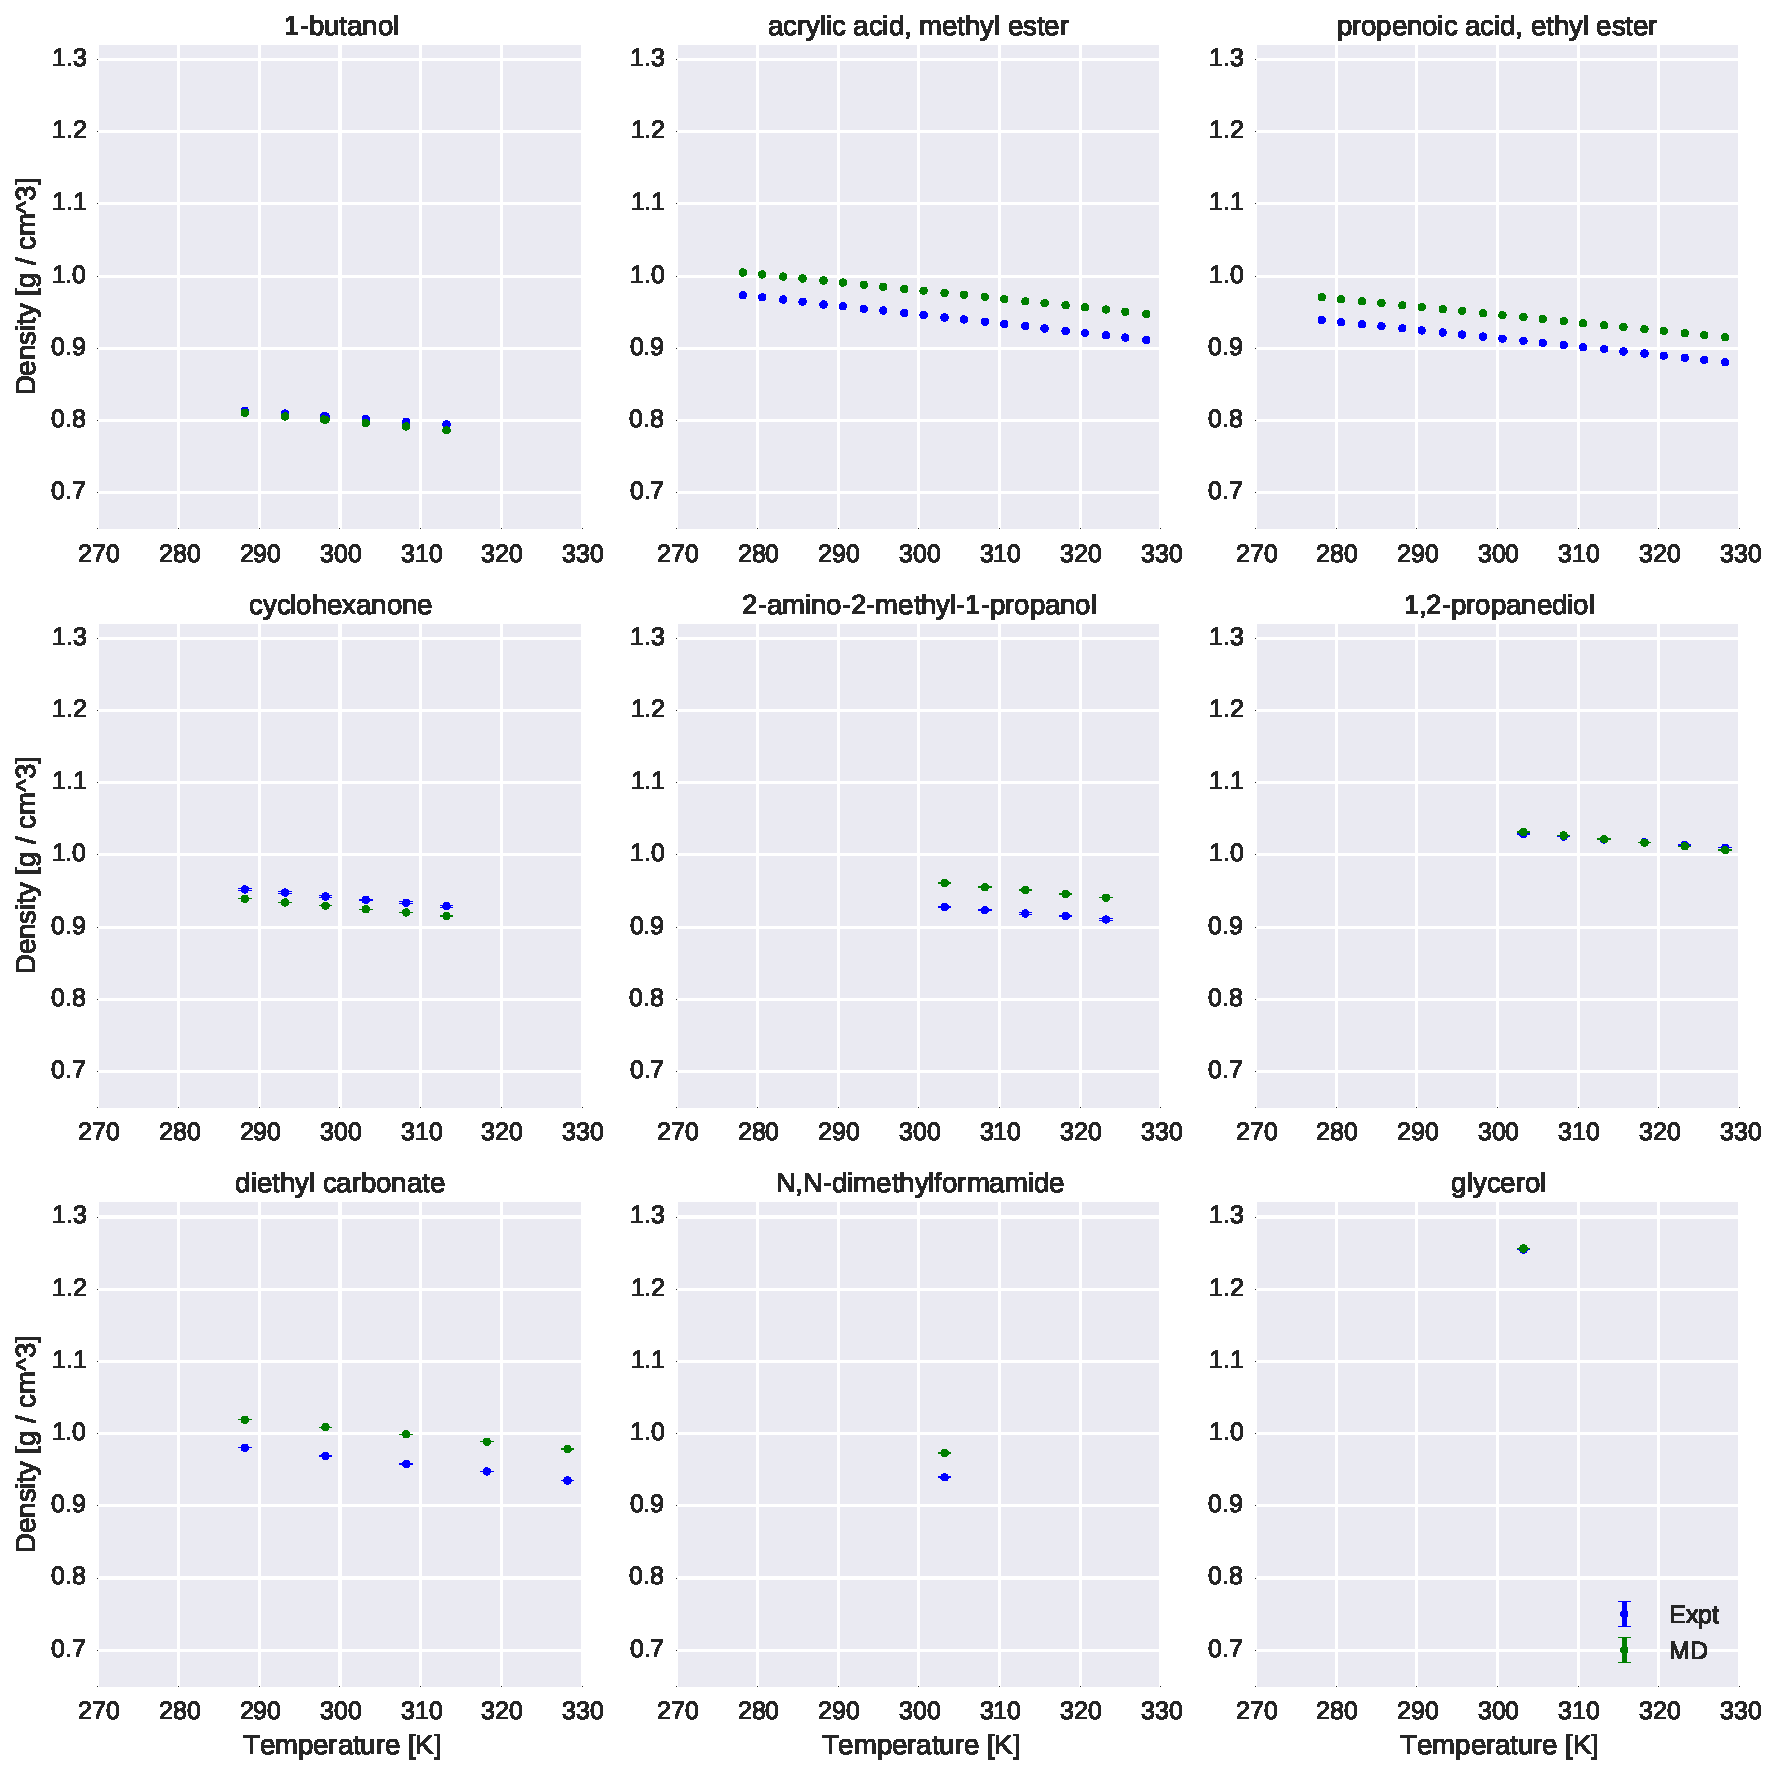
\includegraphics[width=\textwidth]{./figures/densities_versus_temperature_part0.pdf}

\caption{{\bf Comparison of simulated and experimental densities for all compounds.} 
Measured (blue) and simulated (green) densities are shown in units of g/cm$^{3}$.
\label{figure:AllDensities}
}

\end{figure*}

\begin{figure*}[alldensity]


\ContinuedFloat

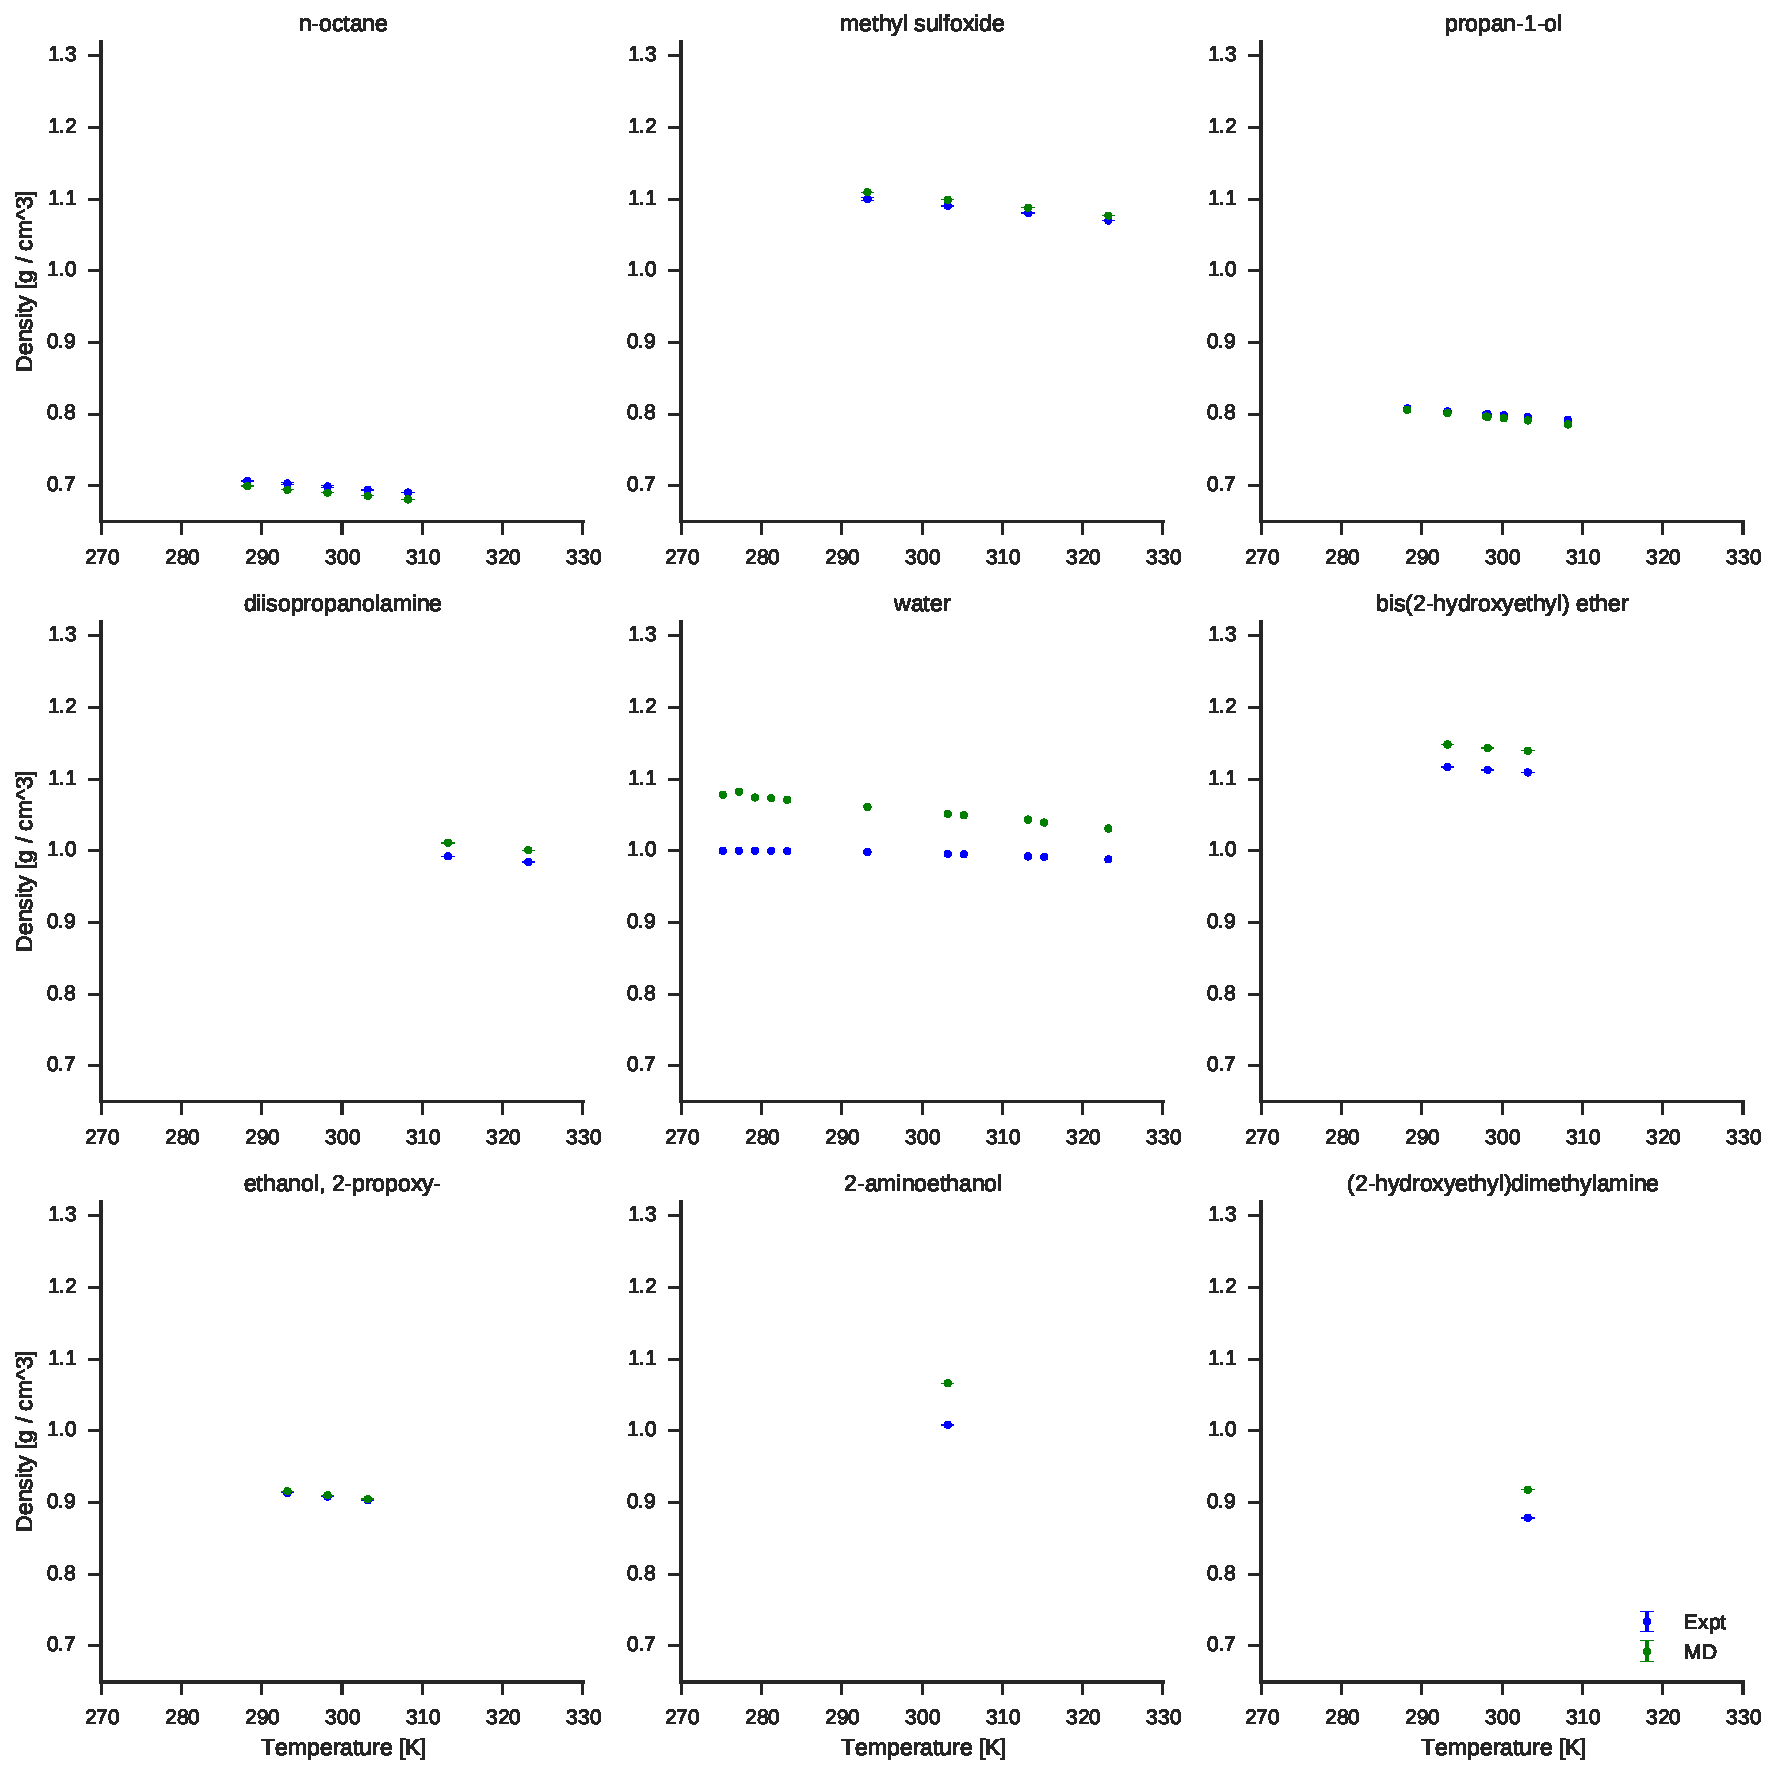
\includegraphics[width=\textwidth]{./figures/densities_versus_temperature_part1.pdf}

\caption{{\bf Comparison of simulated and experimental densities for all compounds.} 
Measured (blue) and simulated (green) densities are shown in units of g/cm$^{3}$.
\label{figure:AllDensities}
}

\end{figure*}

\begin{figure*}[alldensity]

\ContinuedFloat

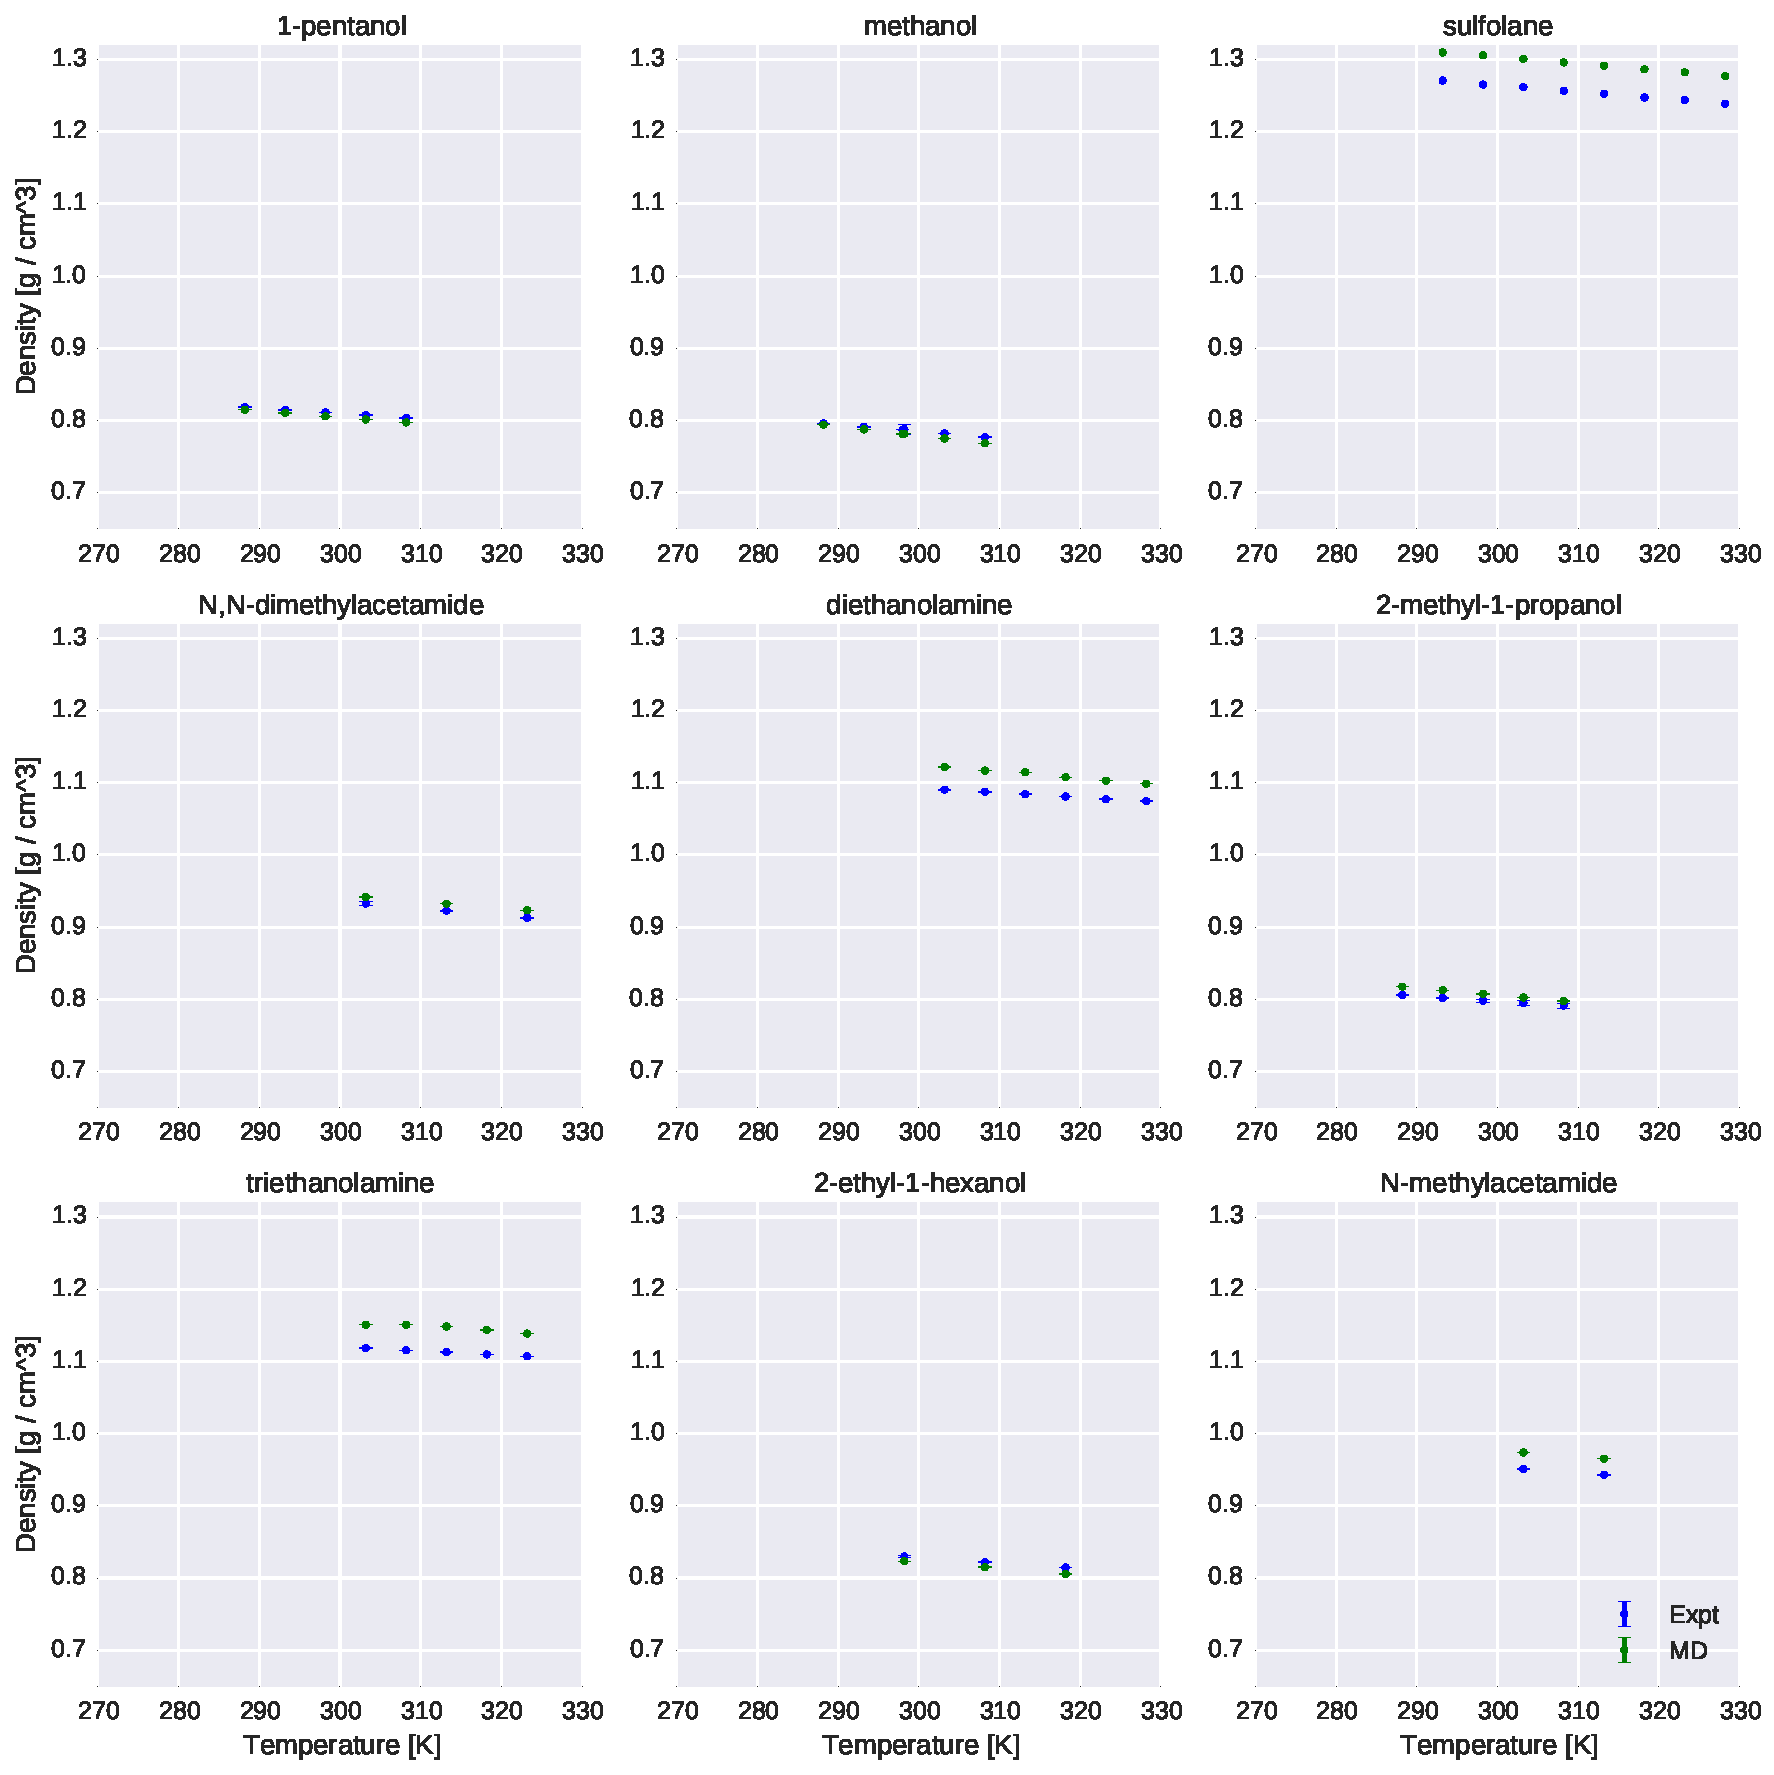
\includegraphics[width=\textwidth]{./figures/densities_versus_temperature_part2.pdf}

\caption{{\bf Comparison of simulated and experimental densities for all compounds.} 
Measured (blue) and simulated (green) densities are shown in units of g/cm$^{3}$.
\label{figure:AllDensities}
}

\end{figure*}


\begin{figure*}[alldensity]

\ContinuedFloat

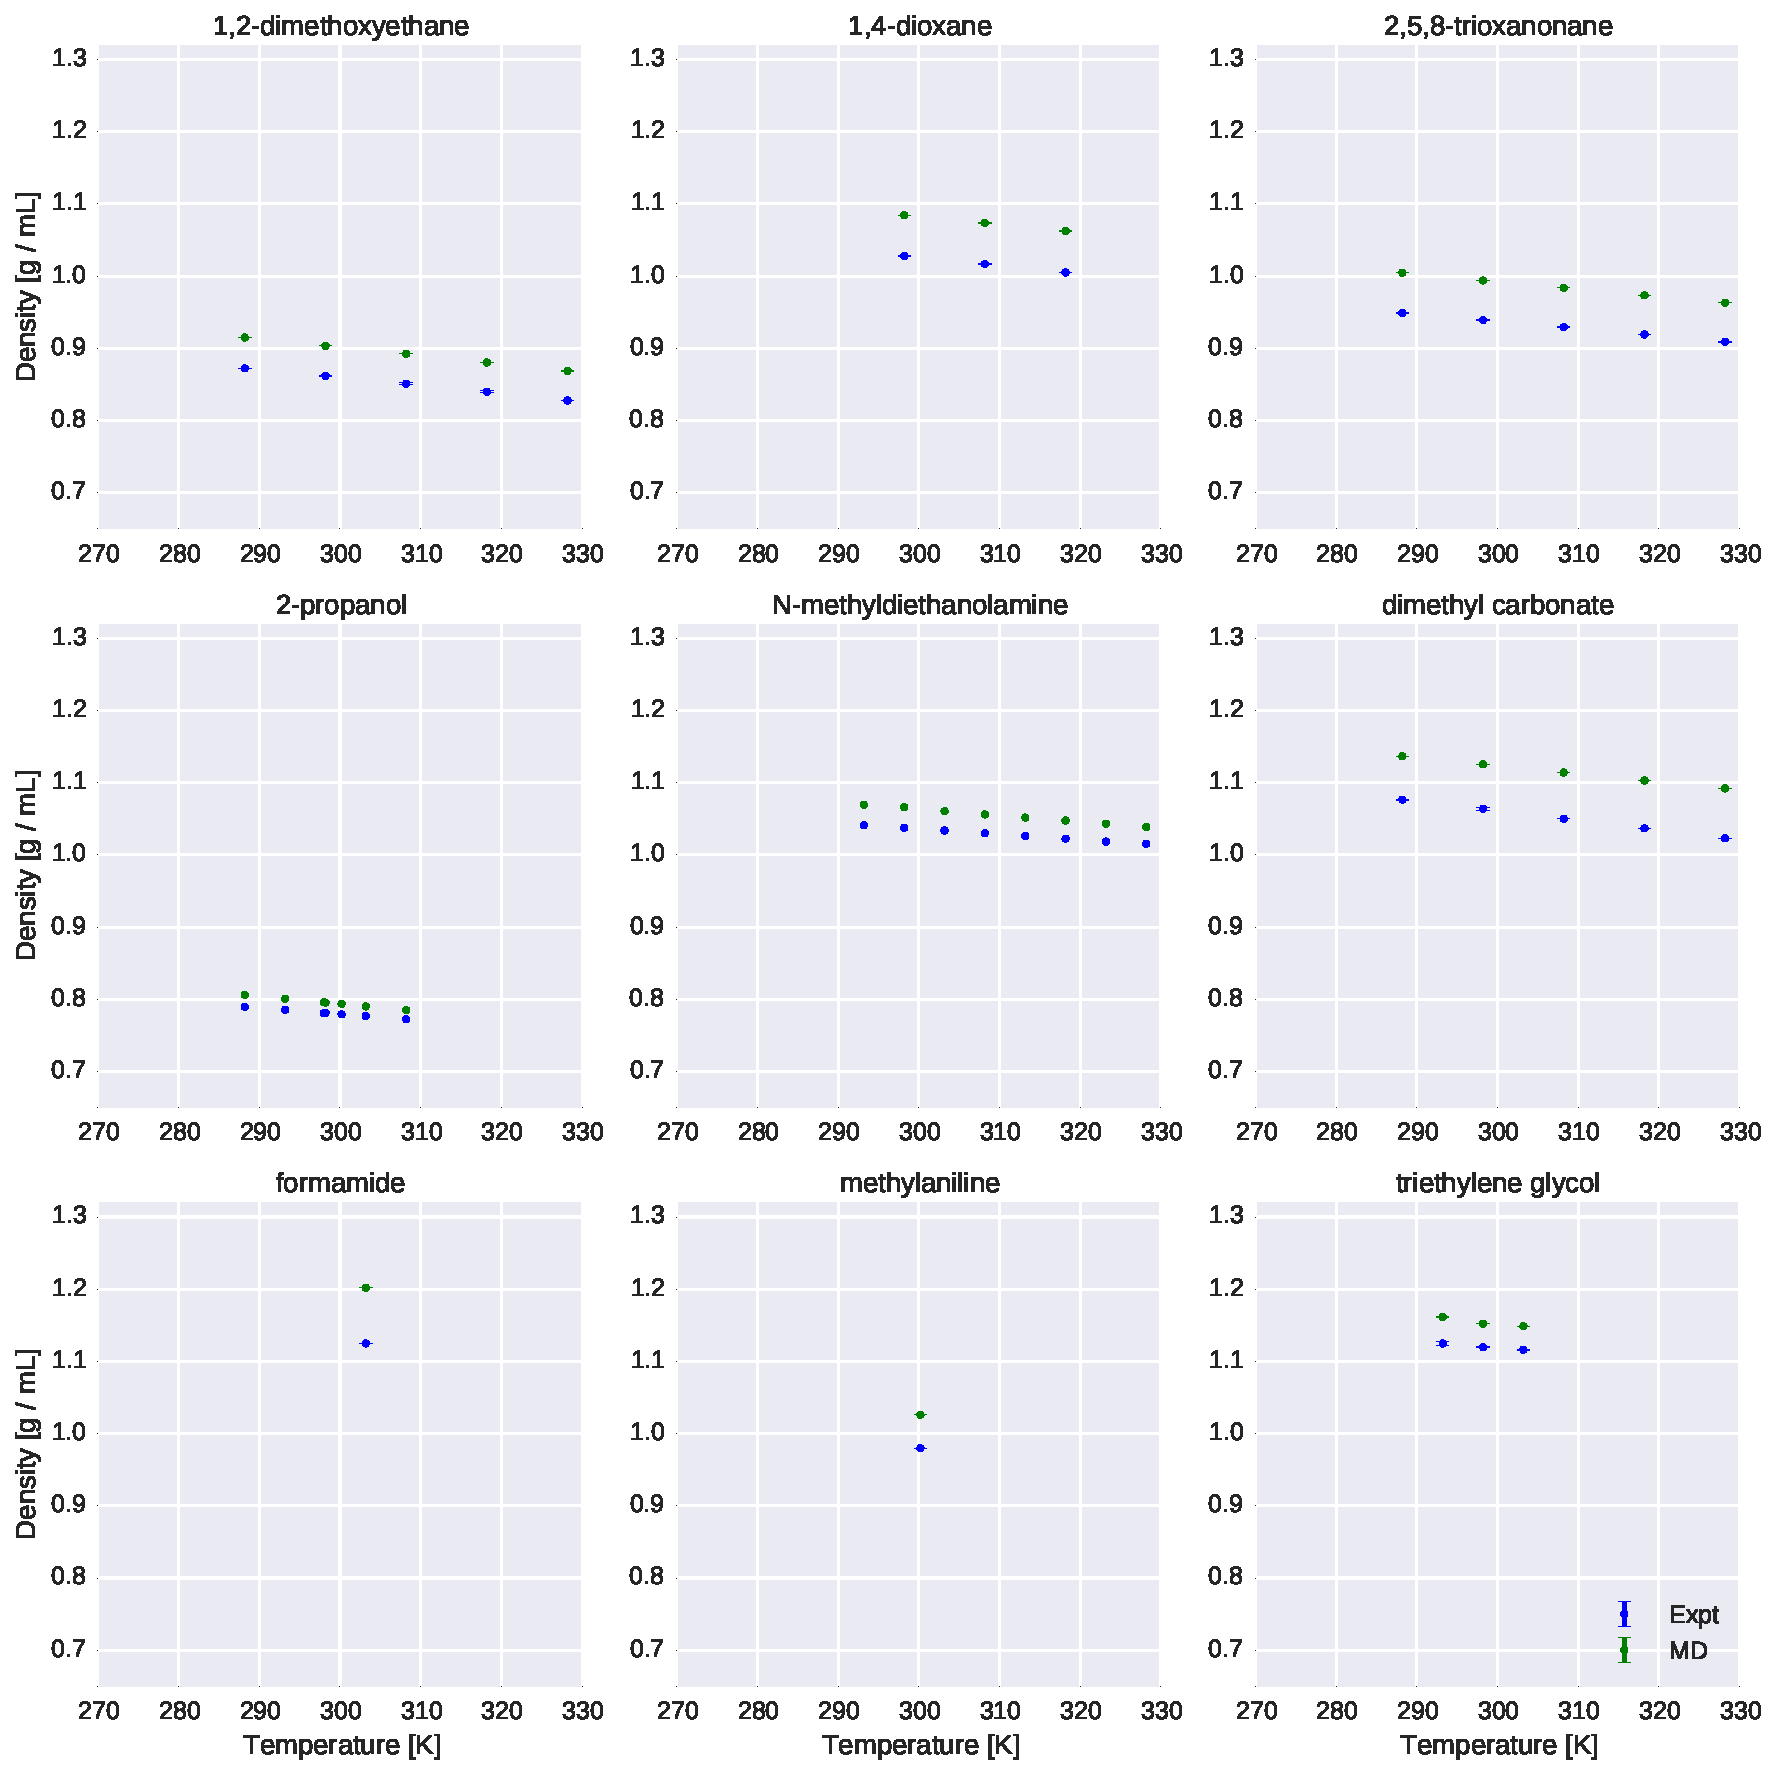
\includegraphics[width=\textwidth]{./figures/densities_versus_temperature_part3.pdf}

\caption{{\bf Comparison of simulated and experimental densities for all compounds.} 
Measured (blue) and simulated (green) densities are shown in units of g/cm$^{3}$.
\label{figure:AllDensities}
}

\end{figure*}


\begin{figure*}[alldensity]

\ContinuedFloat

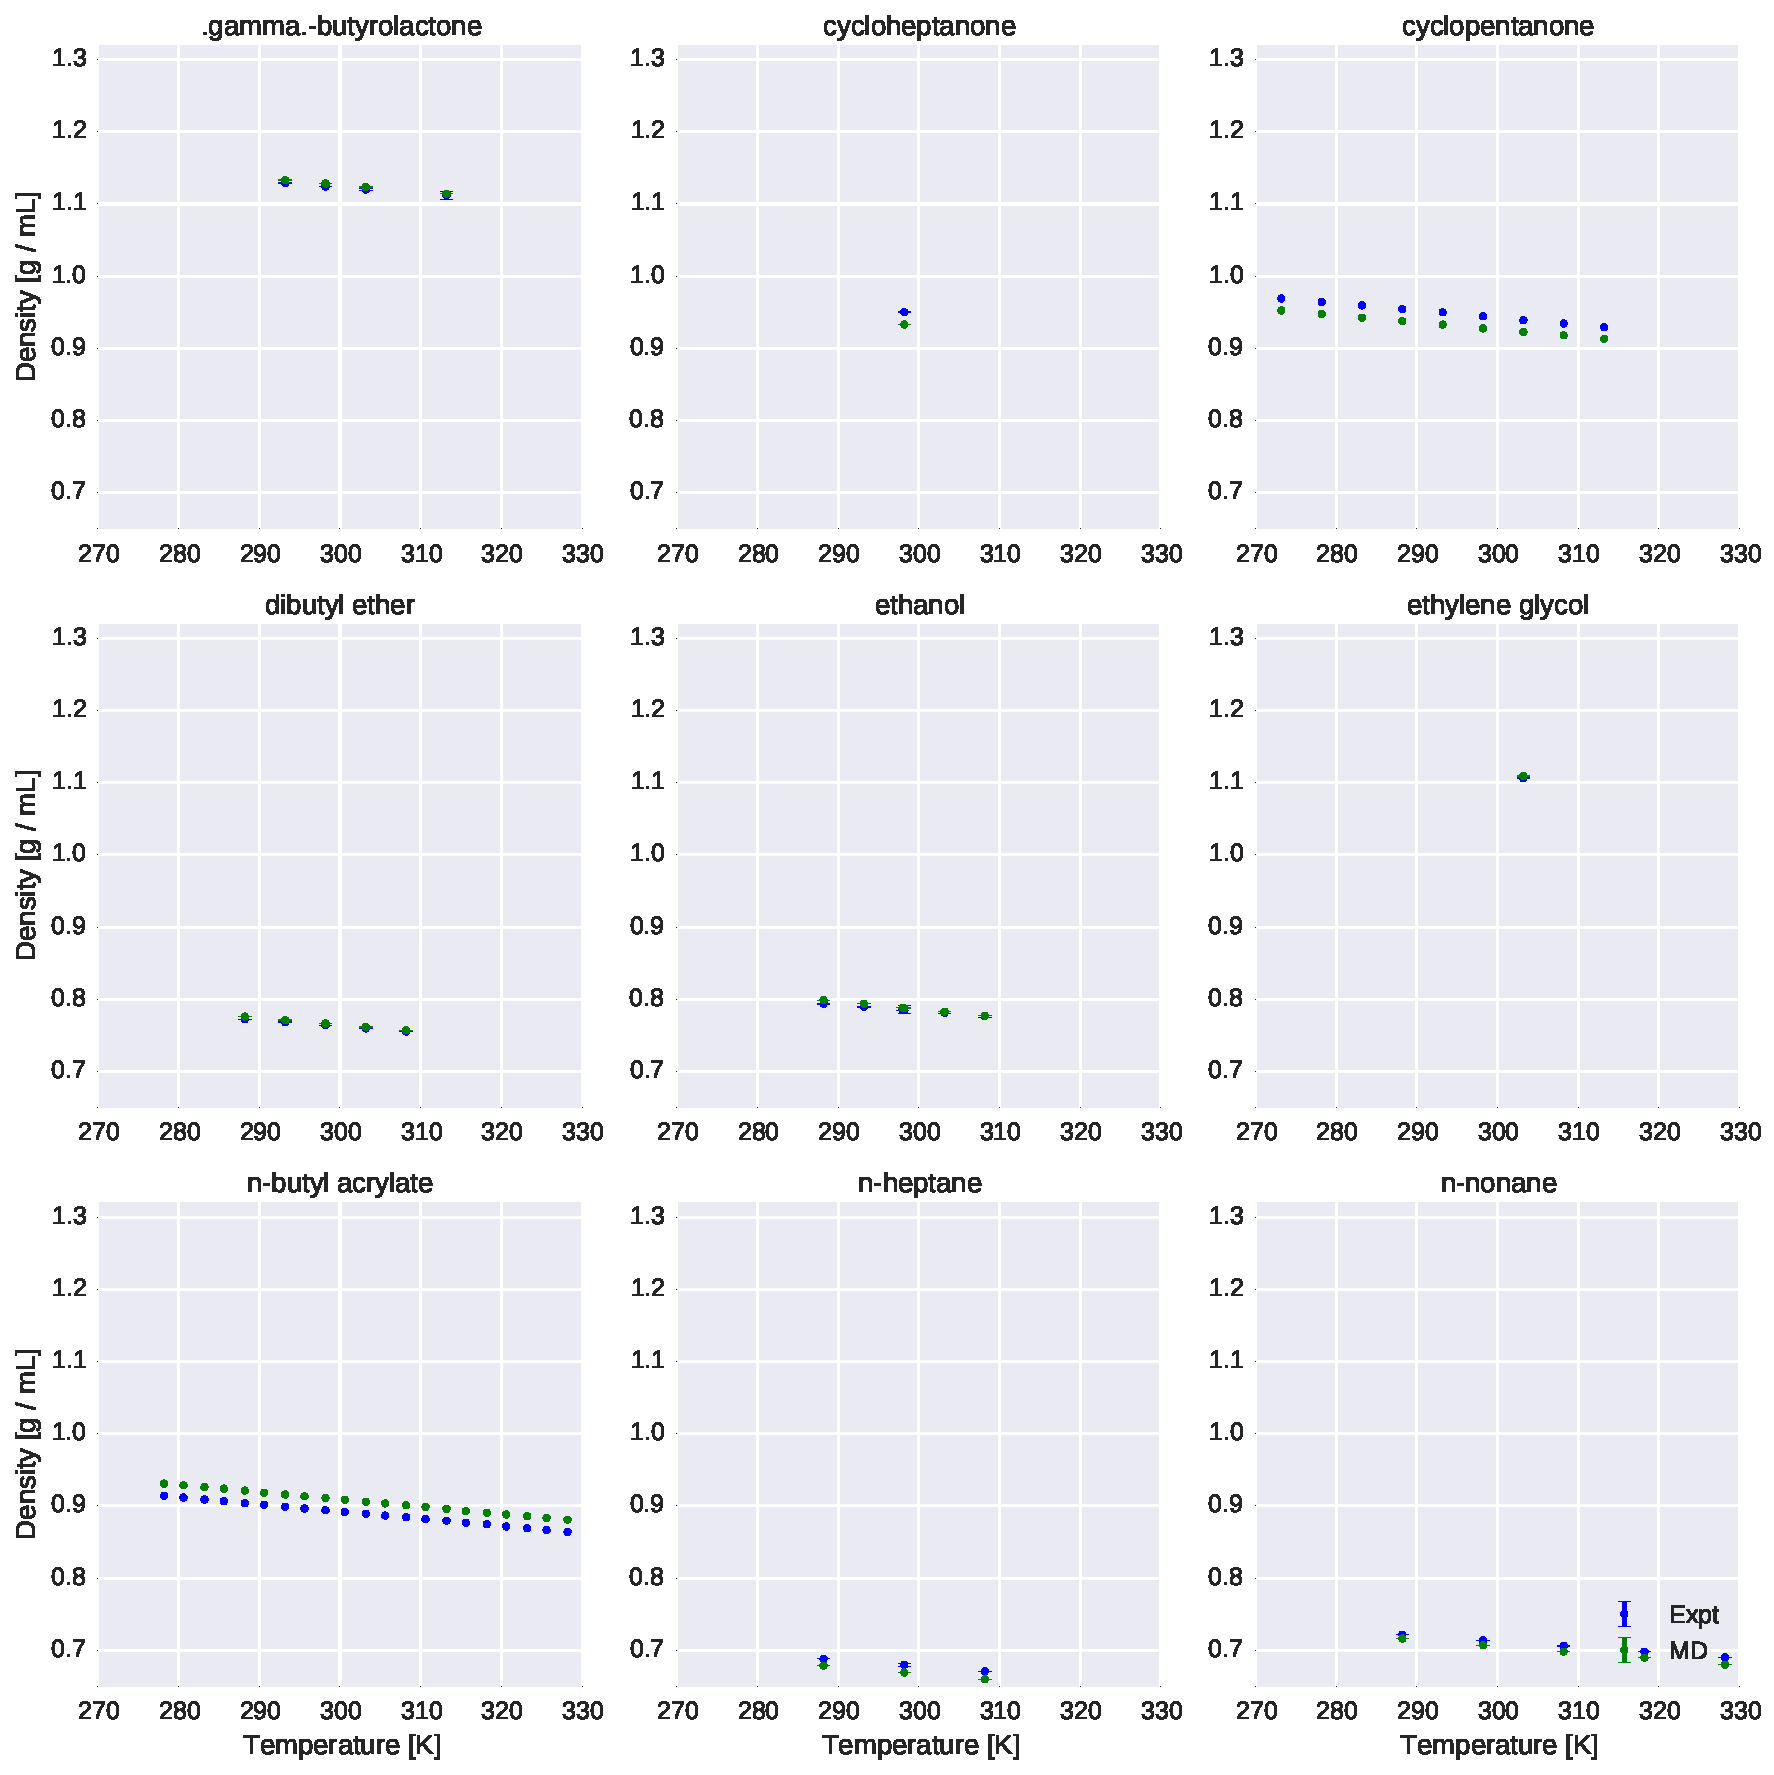
\includegraphics[width=\textwidth]{./figures/densities_versus_temperature_part4.pdf}

\caption{{\bf Comparison of simulated and experimental densities for all compounds.} 
Measured (blue) and simulated (green) densities are shown in units of g/cm$^{3}$.
\label{figure:AllDensities}
}

\end{figure*}



%%%%%%%%%%%%%%%%%%%%%%%%%%%%%%%%%%%%%%%%%%%%%%%%%%%%%%%%%%%%%%%%%%%%%%%%%%%%%%%%
% FIGURE: DIELECTRIC VS TEMPERATURE
%%%%%%%%%%%%%%%%%%%%%%%%%%%%%%%%%%%%%%%%%%%%%%%%%%%%%%%%%%%%%%%%%%%%%%%%%%%%%%%%

\begin{figure*}[alldielectric]

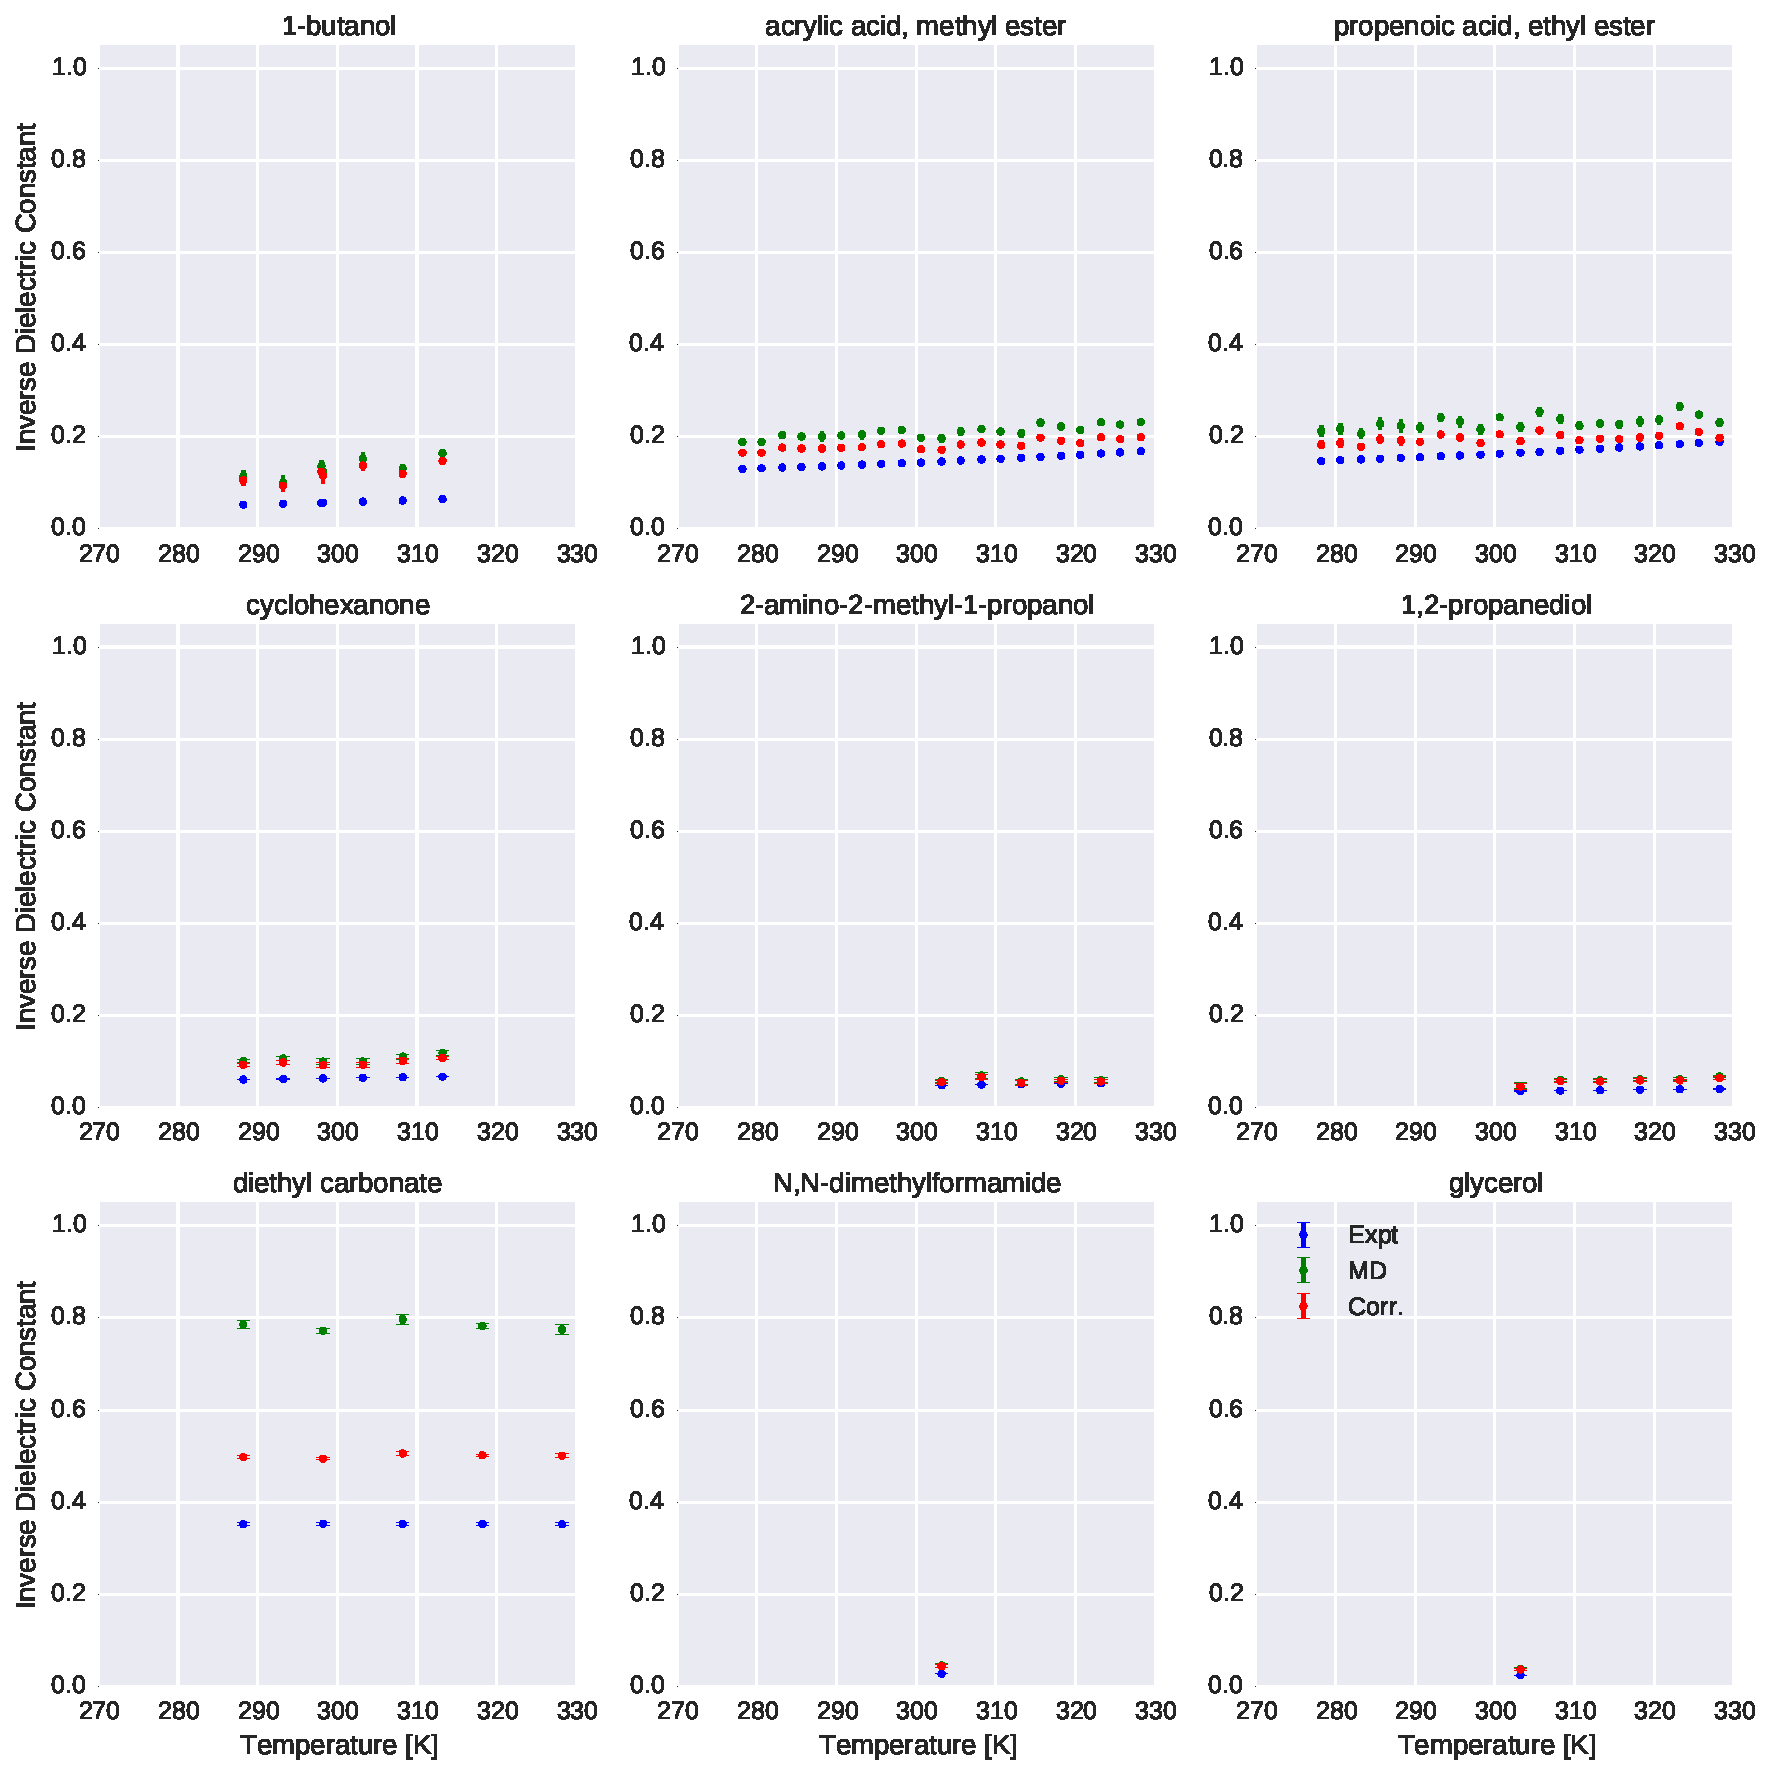
\includegraphics[width=\textwidth]{./figures/dielectric_versus_temperature_part0.pdf}

\caption{{\bf Comparison of simulated and experimental static dielectric constants for all compounds.}
Measured (blue), simulated (green), and polarizability-corrected simulated (red) static dielectric constants are shown for all compounds.
}

\label{figure:AllDielectrics}

\end{figure*}


\begin{figure*}[alldielectric]

\ContinuedFloat

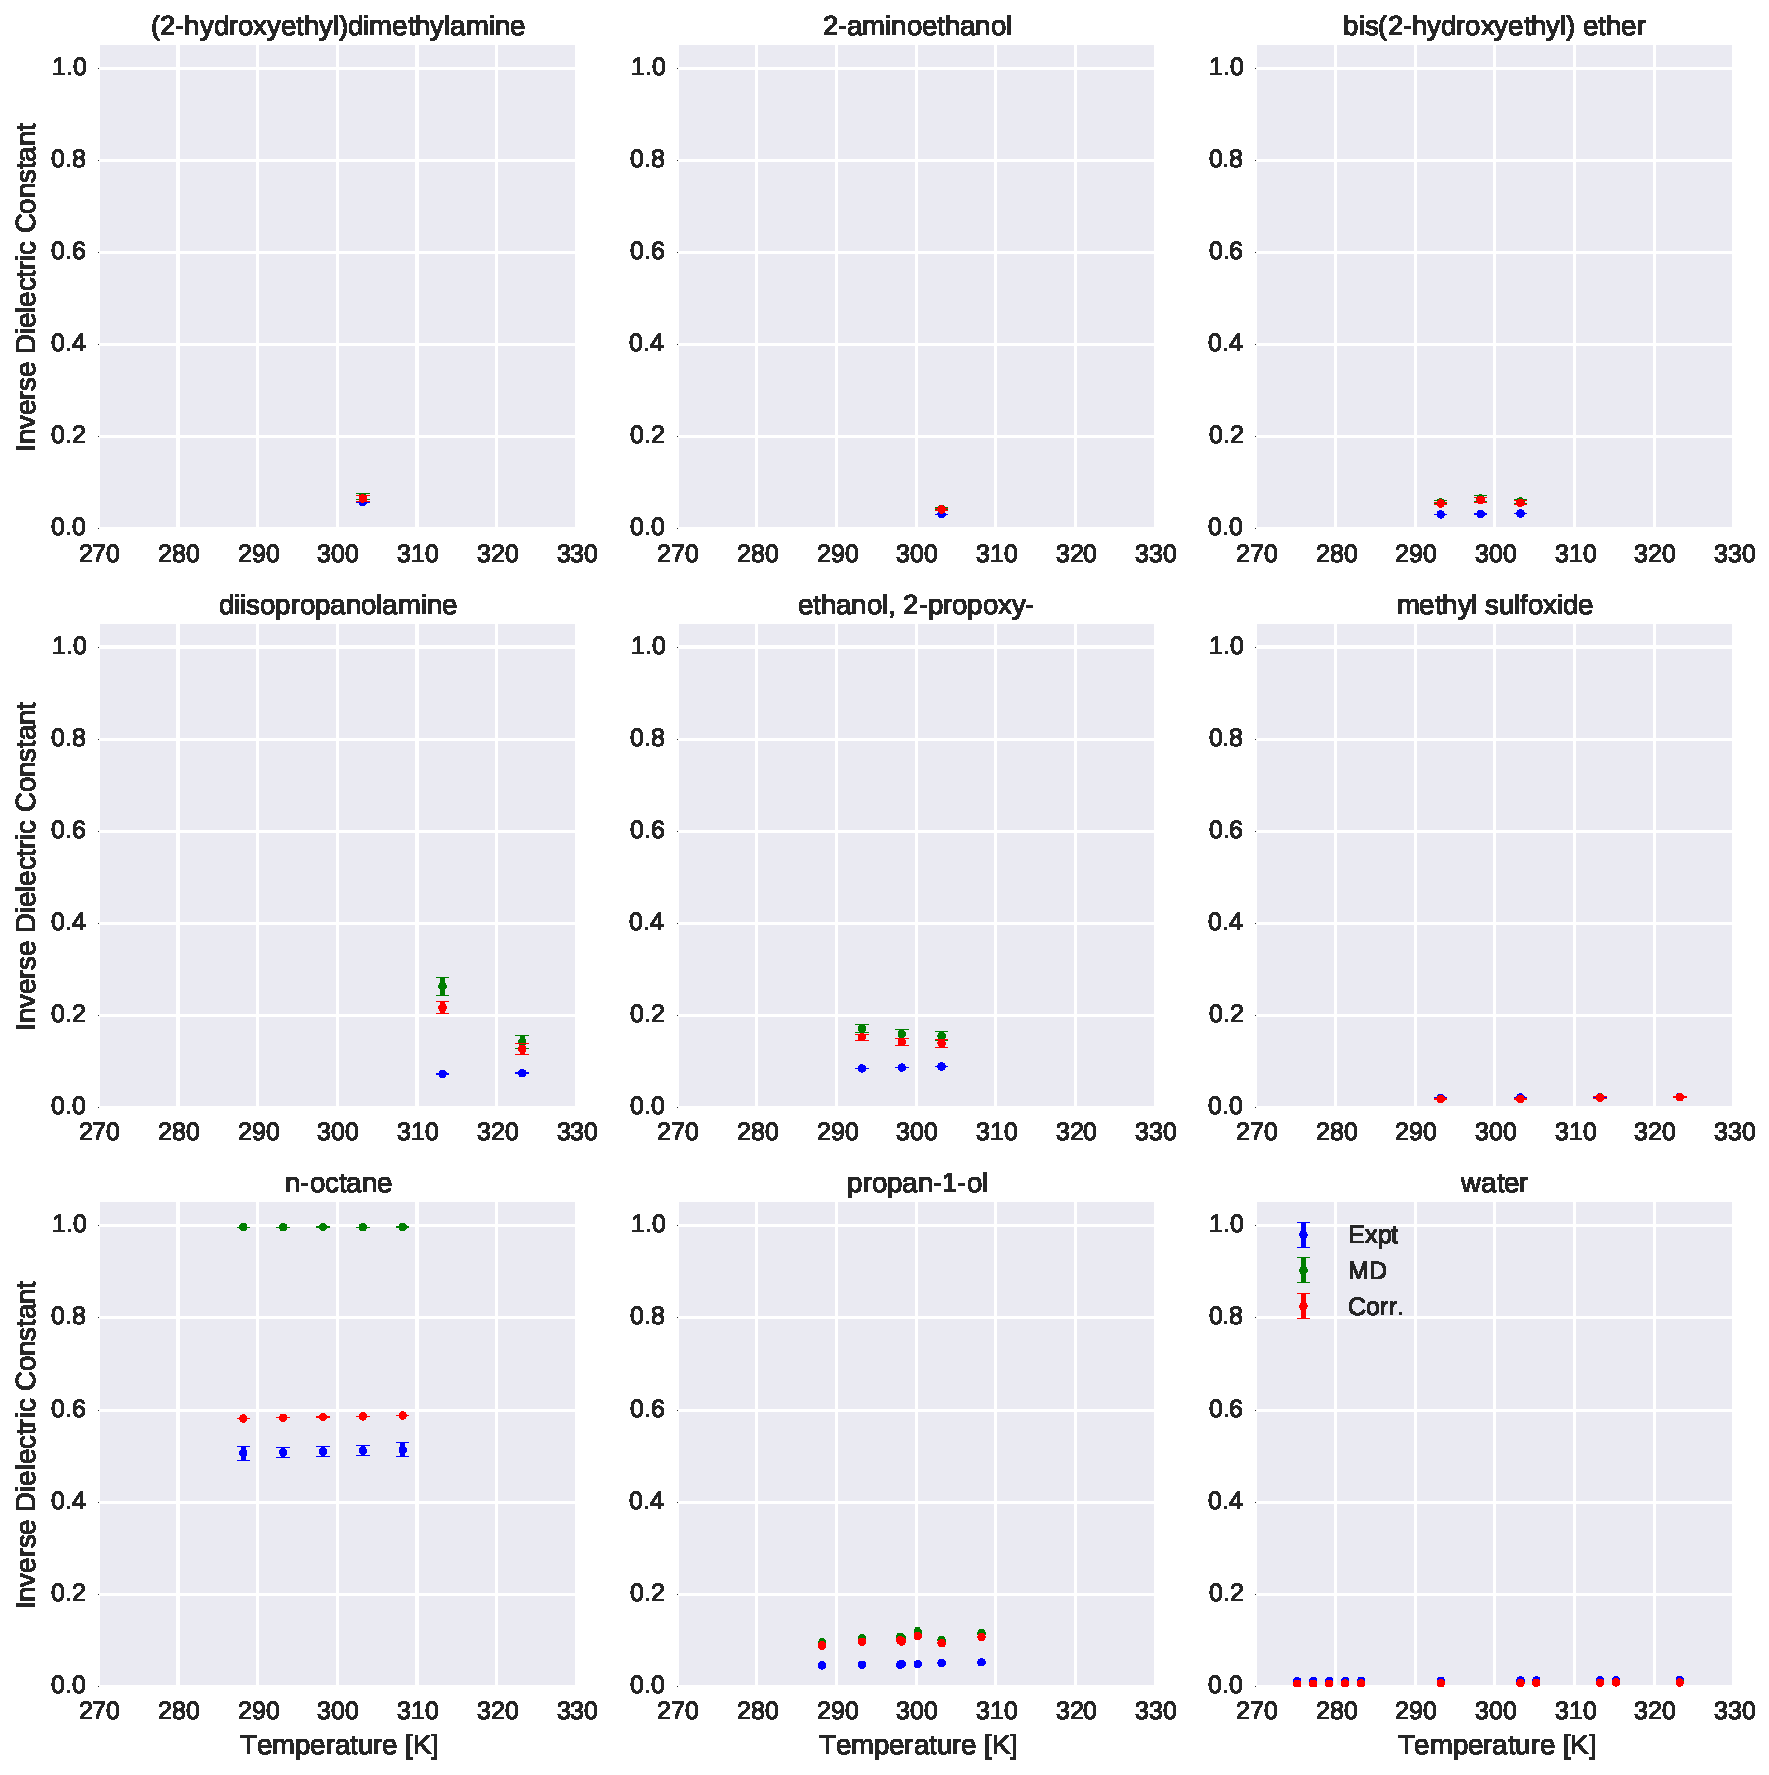
\includegraphics[width=\textwidth]{./figures/dielectric_versus_temperature_part1.pdf}

\caption{{\bf Comparison of simulated and experimental static dielectric constants for all compounds.}
Measured (blue), simulated (green), and polarizability-corrected simulated (red) static dielectric constants are shown for all compounds.
}

\label{figure:AllDielectrics}

\end{figure*}

\begin{figure*}[alldielectric]

\ContinuedFloat

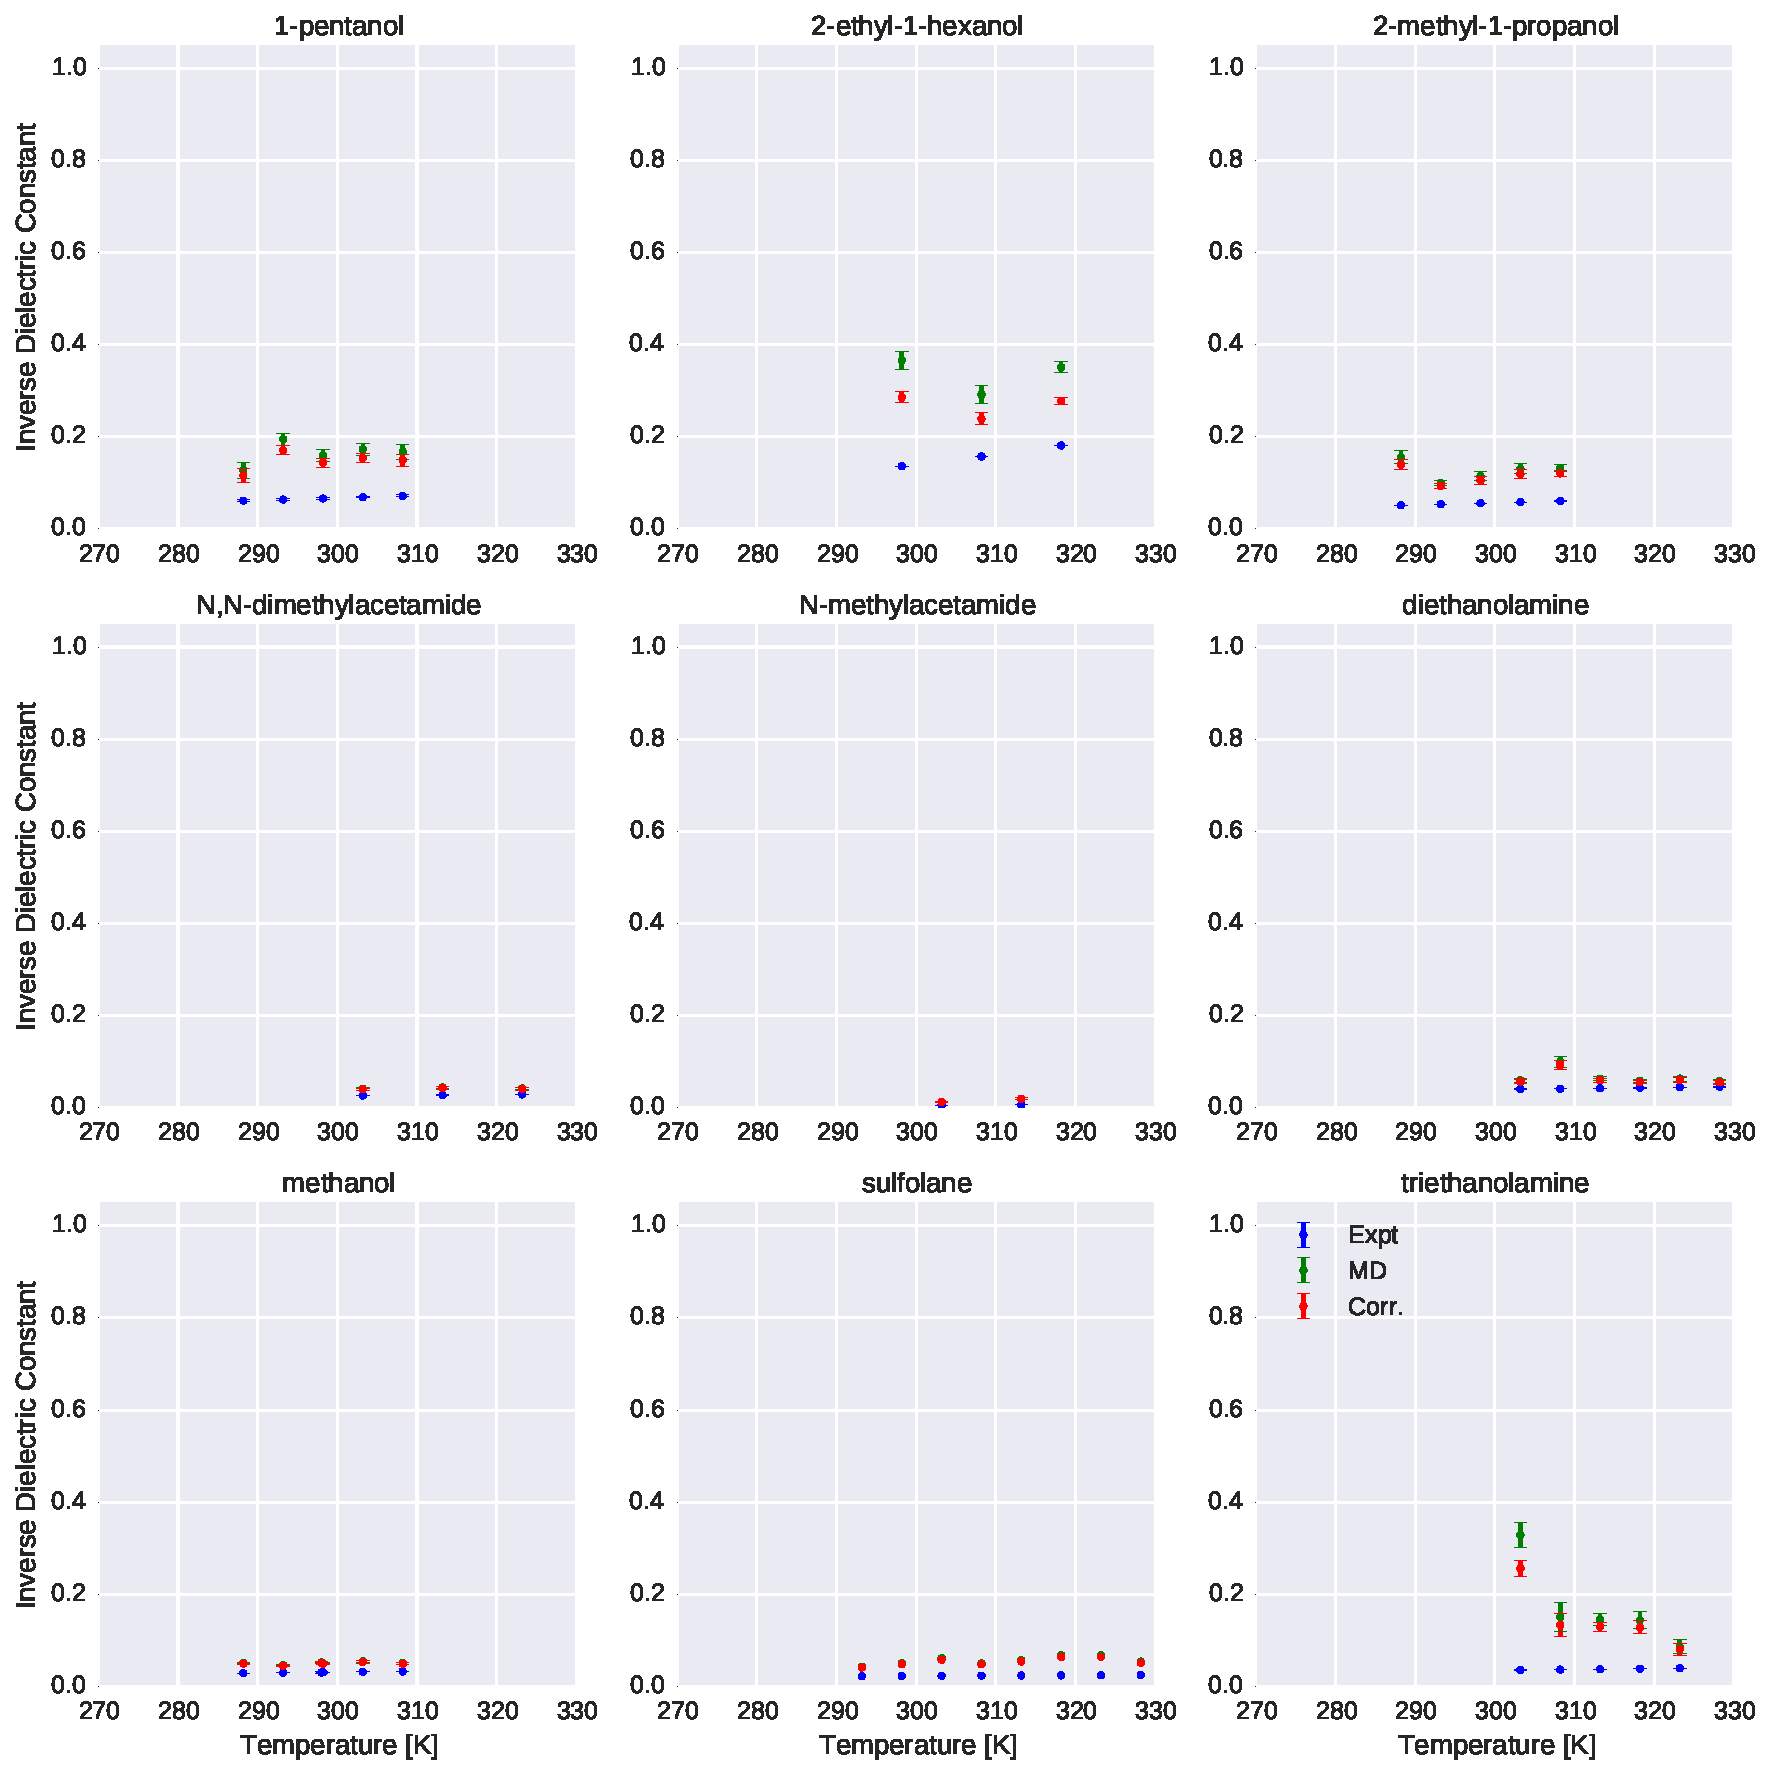
\includegraphics[width=\textwidth]{./figures/dielectric_versus_temperature_part2.pdf}

\caption{{\bf Comparison of simulated and experimental static dielectric constants for all compounds.}
Measured (blue), simulated (green), and polarizability-corrected simulated (red) static dielectric constants are shown for all compounds.
}

\label{figure:AllDielectrics}

\end{figure*}

\begin{figure*}[alldielectric]

\ContinuedFloat

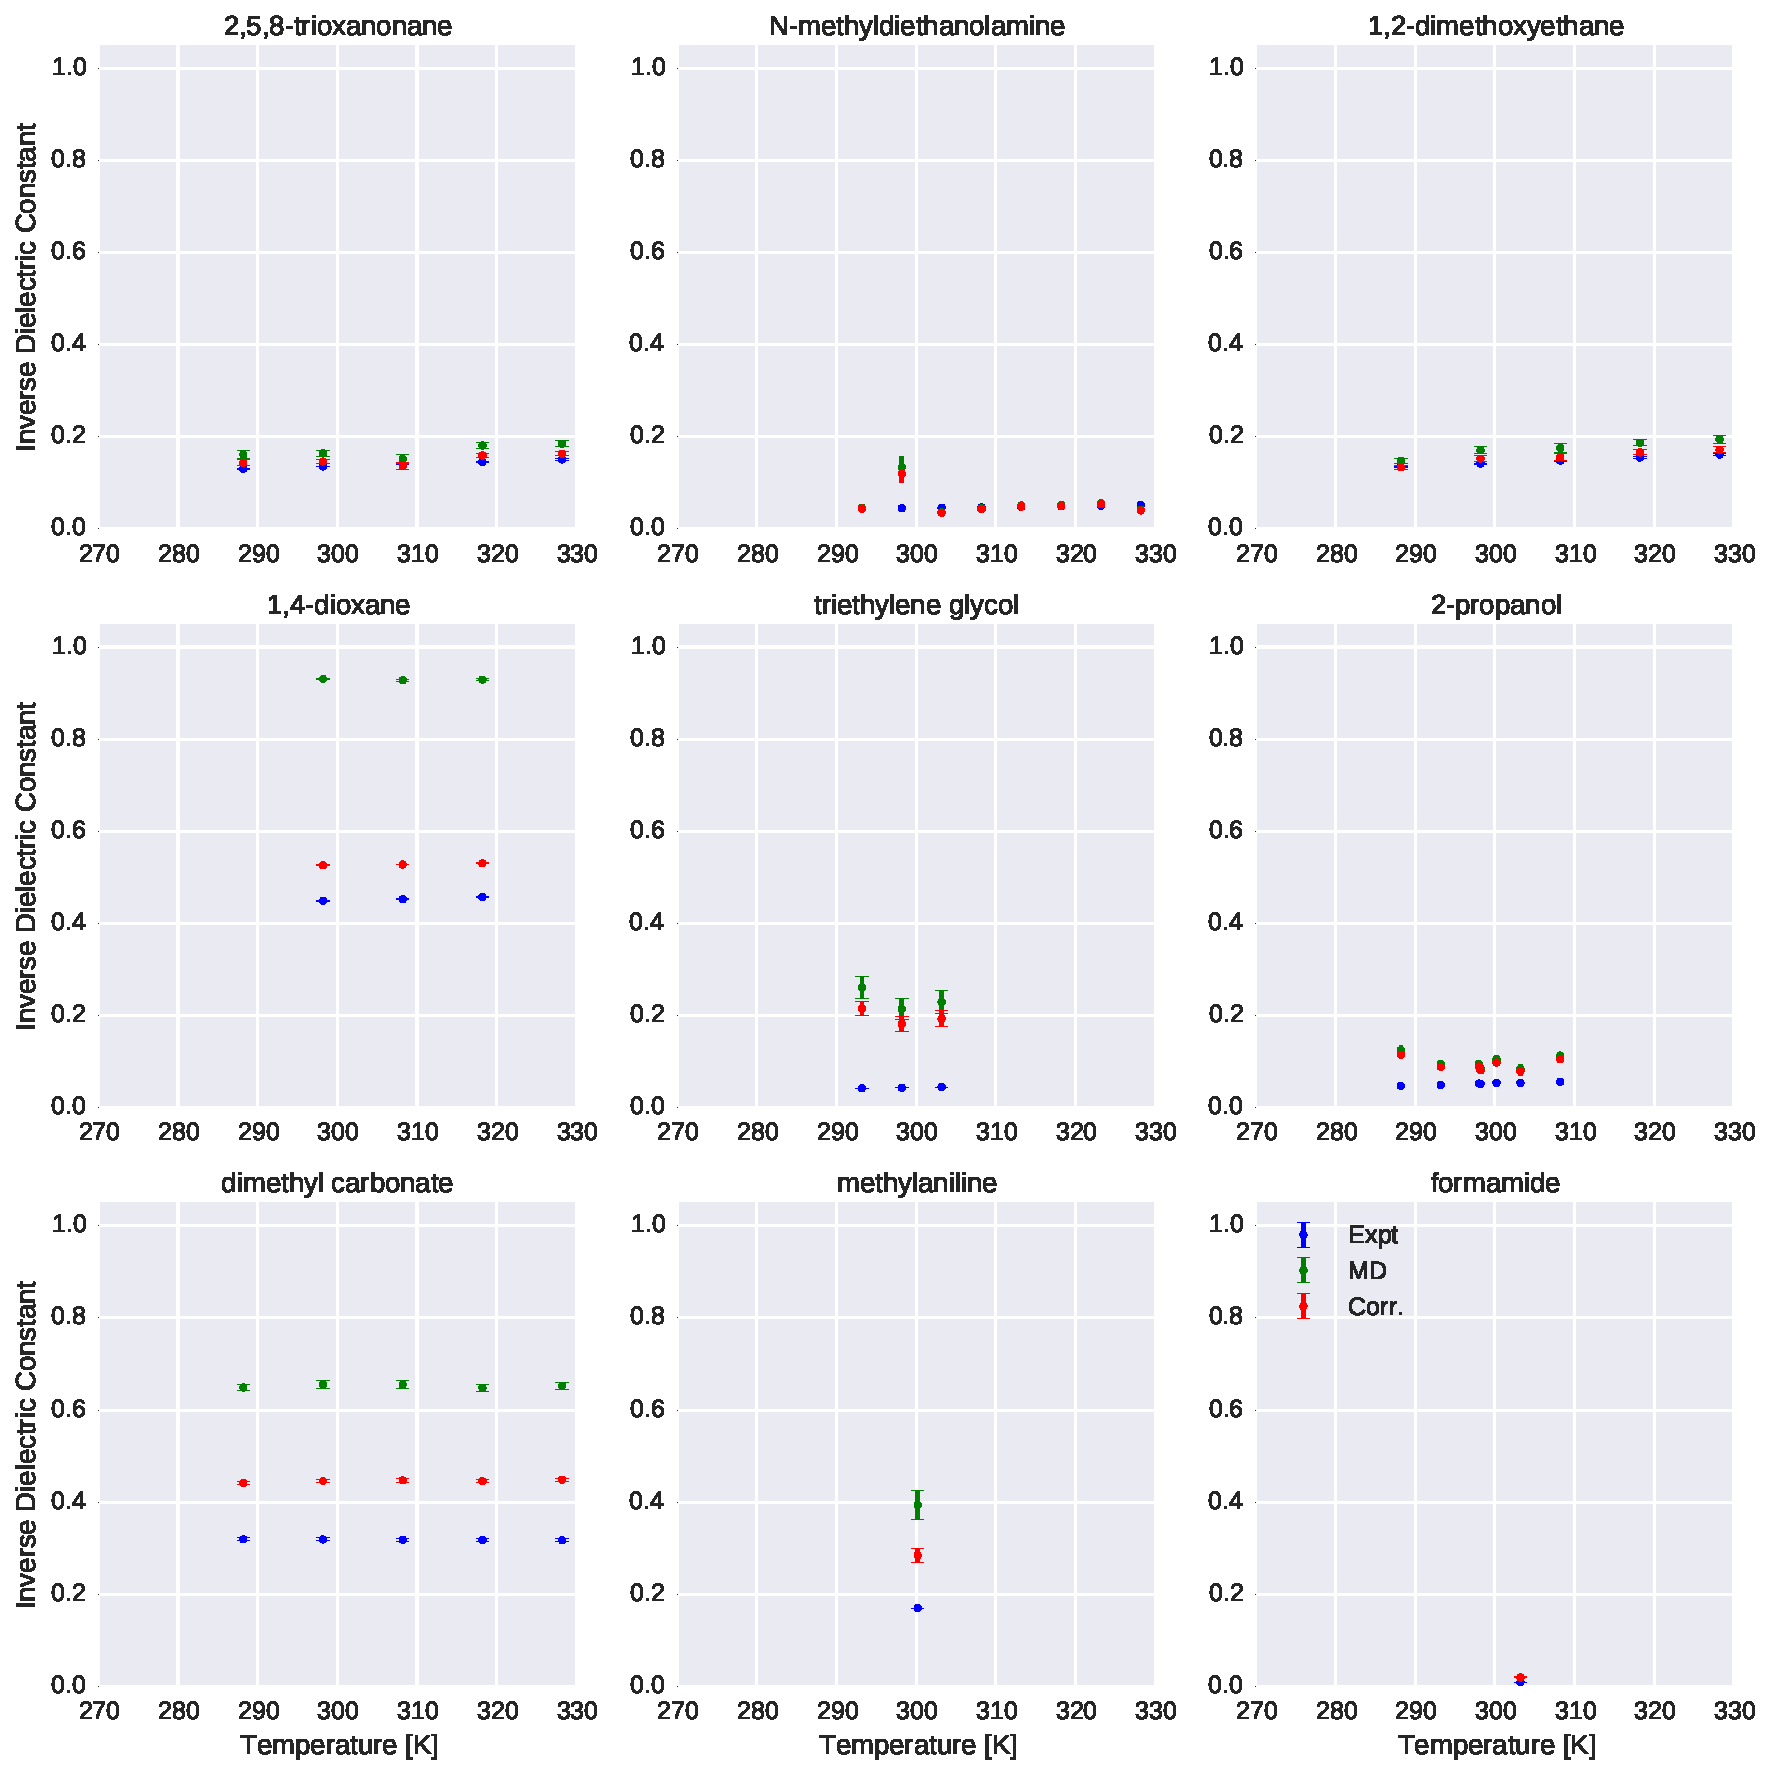
\includegraphics[width=\textwidth]{./figures/dielectric_versus_temperature_part3.pdf}

\caption{{\bf Comparison of simulated and experimental static dielectric constants for all compounds.}
Measured (blue), simulated (green), and polarizability-corrected simulated (red) static dielectric constants are shown for all compounds.
}

\label{figure:AllDielectrics}

\end{figure*}

\begin{figure*}[alldielectric]

\ContinuedFloat

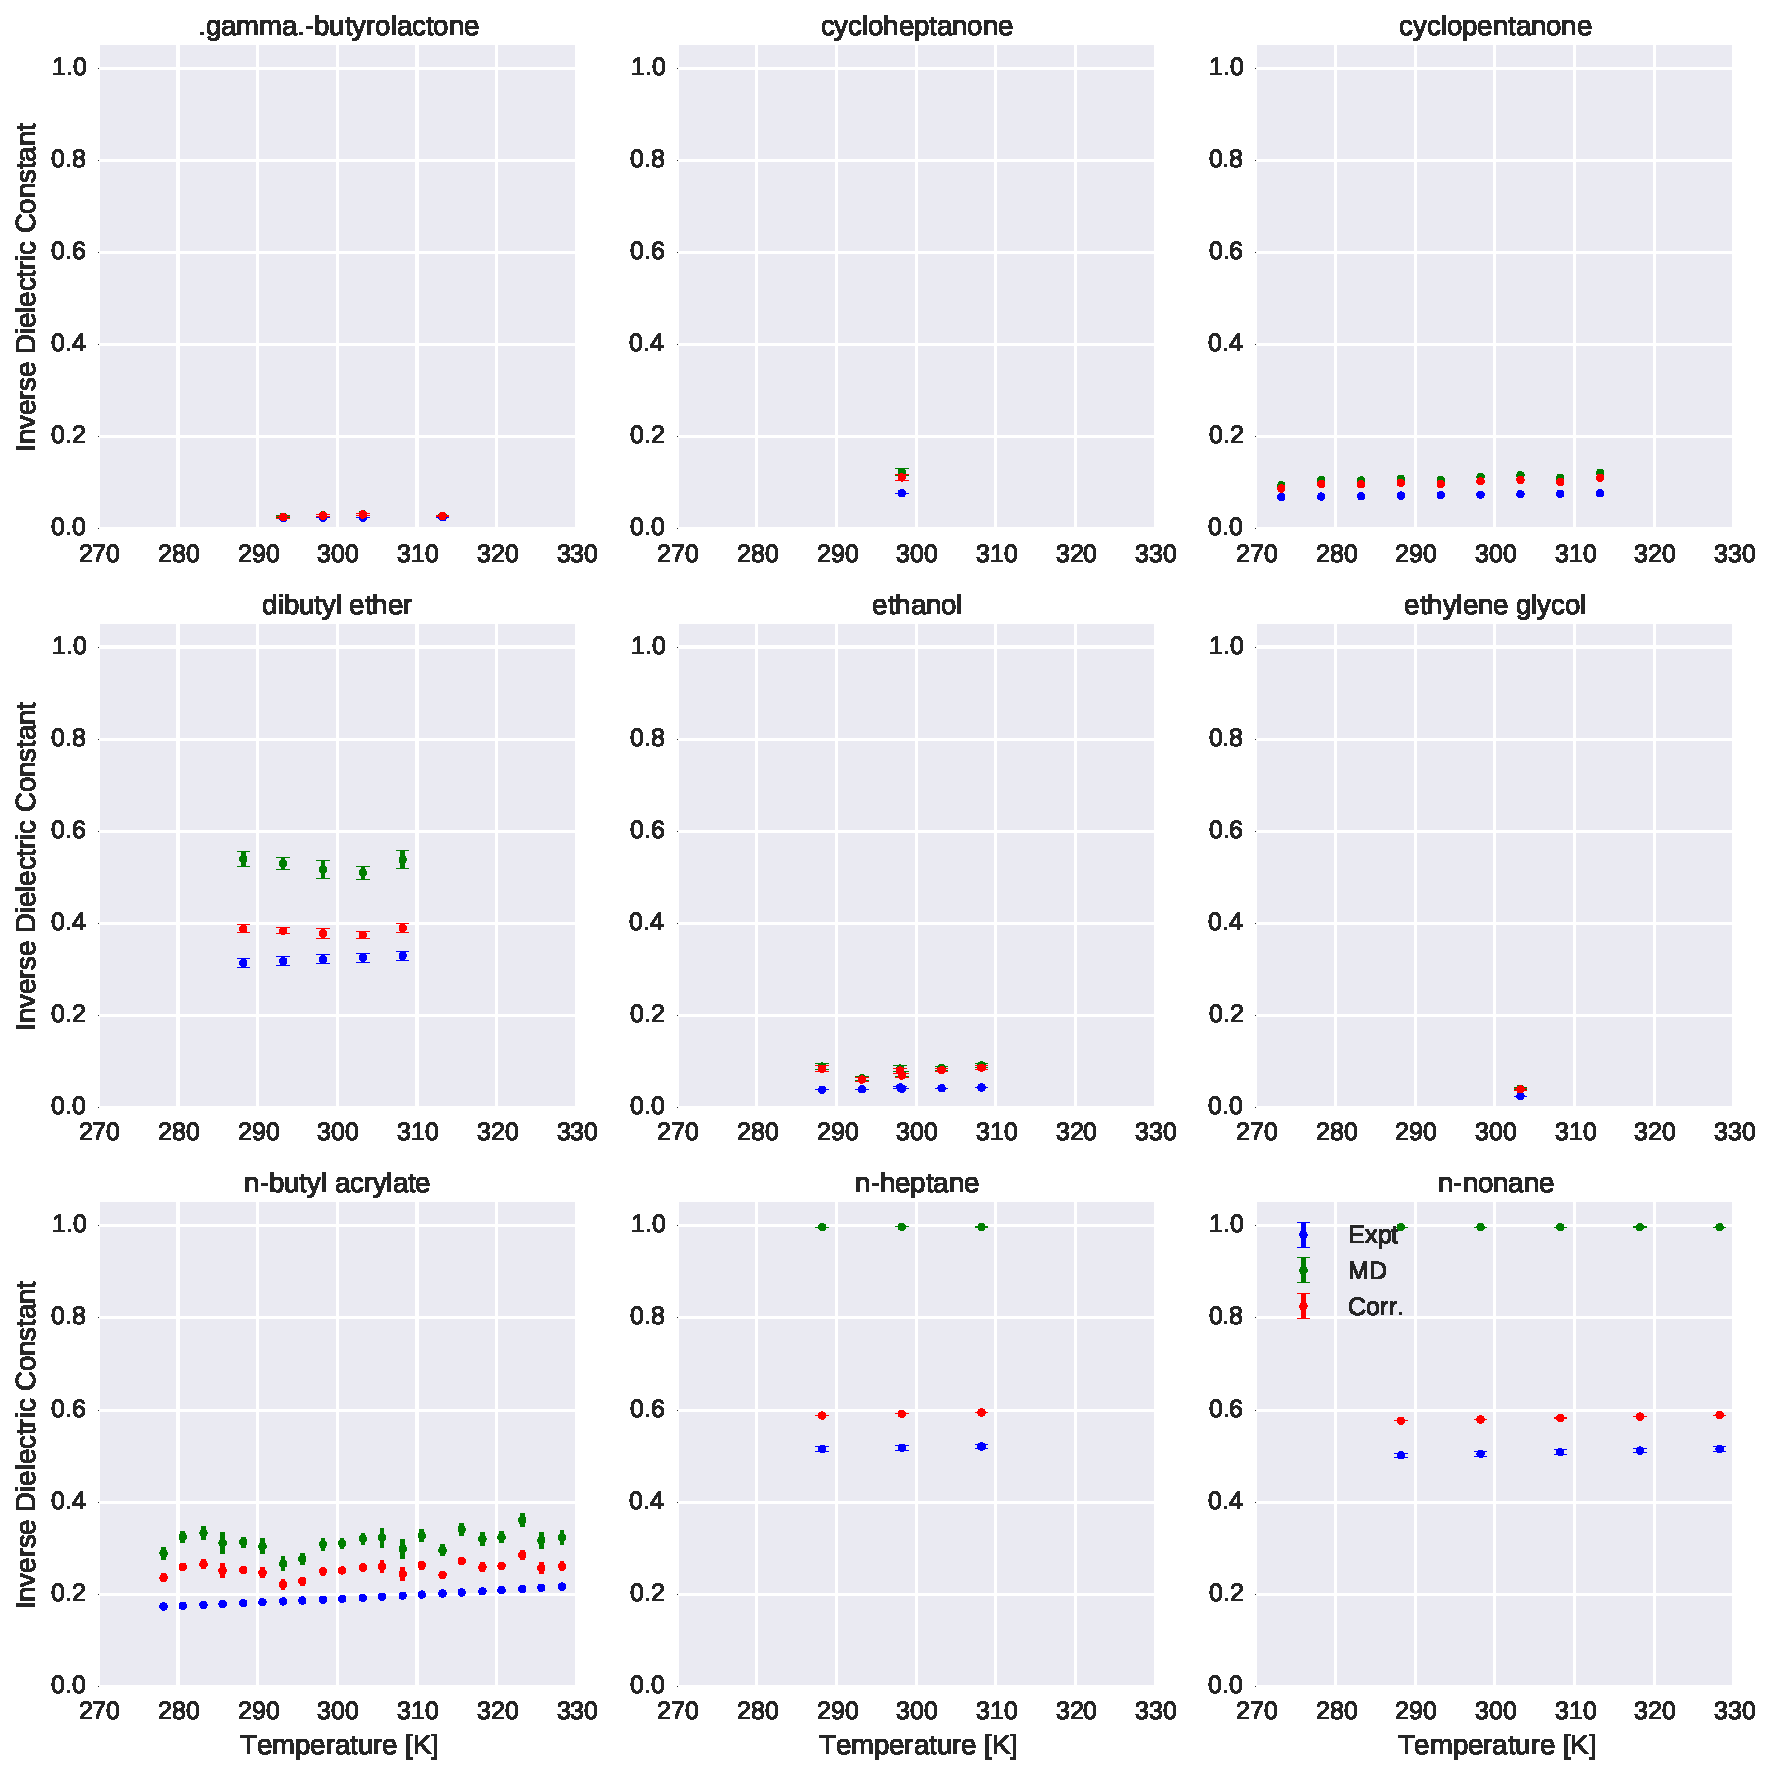
\includegraphics[width=\textwidth]{./figures/dielectric_versus_temperature_part4.pdf}

\caption{{\bf Comparison of simulated and experimental static dielectric constants for all compounds.}
Measured (blue), simulated (green), and polarizability-corrected simulated (red) static dielectric constants are shown for all compounds.
}

\label{figure:AllDielectrics}

\end{figure*}






\clearpage


\subsection{Dependency Installation}
\label{section:commands}

The following shell commands can be used to install the necessary prerequisites via the {\tt conda} package manager for Python:

\begin{lstlisting}[language=bash]
$ conda config --add channels http://conda.binstar.org/omnia
$ conda install "openmoltools" "pymbar==2.1" "mdtraj==1.3" "openmm==6.3" packmol
%\end{lstlisting}

Note that this command installs the exact versions used in the present study, with the exception of openmoltools for which only a more recent package is available.  
However, for authors interested in extending the present work, we suggust using the most up-to-date versions available instead, which involves replacing the equality symbols $==$ with $>=$.


\clearpage

\bibliography{benchmark}

\end{document}
